\documentclass[tikz,crop,convert={density=200,outext=.png},border=0.4cm]{standalone}

\usepackage{pgfplots}
\usepackage{amsmath}
\usetikzlibrary{arrows.meta}
\usepackage{physics}
\usepackage{xcolor}
\definecolor{mixed_1}{RGB}{2,56,88}
\definecolor{mixed_2}{RGB}{54,144,192}
\definecolor{mixed_3}{RGB}{208,209,230}
\pgfplotsset{compat=newest,
    %width=6cm,
    %height=3cm,
    scale only axis=true,
    max space between ticks=25pt,
    try min ticks=5,
    every axis/.style={
        axis y line=middle,
        axis x line=middle,
        axis line style={thick,->,>=latex, shorten >=-.3cm}
    },
    every axis plot/.append style={thick},
    tick style={black, thick},
}
\tikzset{
    semithick/.style={line width=0.8pt},
}
\usepgfplotslibrary{groupplots}
\usepgfplotslibrary{dateplot}
% Document begins
\begin{document}
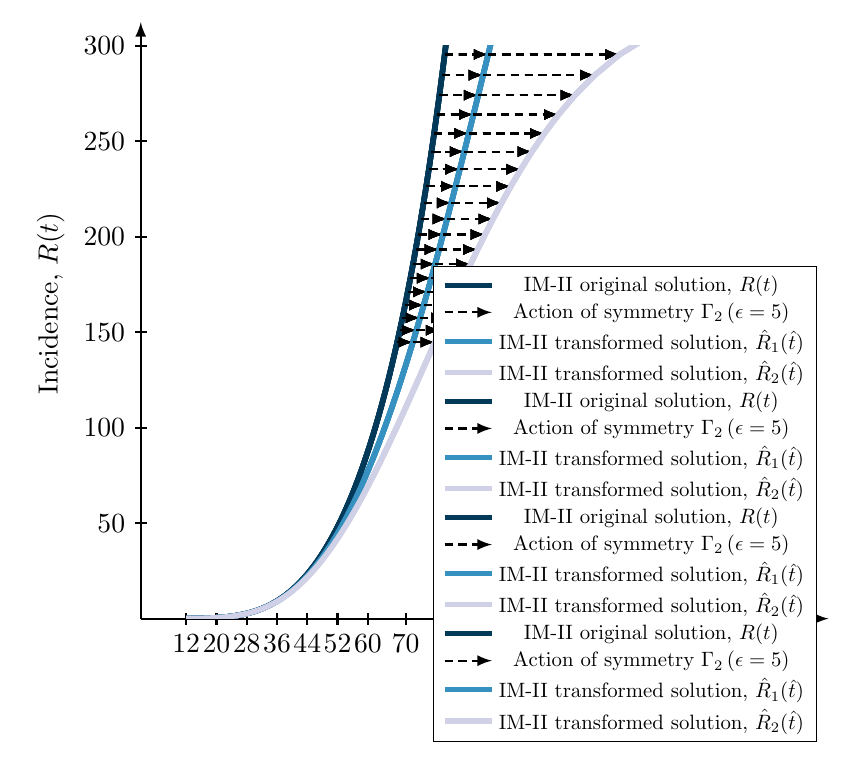
\begin{tikzpicture}
  % The axis of the plot
\begin{axis}[
    %title={Model: $\dv{y}{t}=\frac{2y}{t}$ with solution $y(t)=C_1t^2$\\Symmetry: $\Gamma_{\epsilon}=(t,y)\mapsto\left(\exp\left(\epsilon\right)t,\exp\left(-\epsilon\right)y\right)$},
    title style = {align=left},
    xlabel={Age, $t$},
    ylabel={Incidence, $R(t)$},
    %ylabel={Logarithm of Incidence, $\ln\left(R(t)\right)$},        
    x label style={at={(axis description cs:0.5,-0.1)},anchor=north},
    y label style={at={(axis description cs:-0.1,0.55)},rotate=90,anchor=south},    
    xmin=0, xmax=175.5,
    % xmin=-27, xmax=5,
    ymin=0, ymax=300,
    %xtick={-30,-27,...,9},
    xtick={0,12,20,...,60,70,82,90,100,150},    
    %ytick={-15,-10,...,15},
    legend style={at={(axis description cs:0.44,0.2)},anchor=west,nodes={scale=0.75, transform shape}},    
    %legend pos=north west,
    %ymajorgrids=true,
    grid style=dashed,
]
% Plot the data
\addplot[
color=mixed_1,line width=2pt,
]
coordinates {%
(12.0,0.044124524681051186)
(12.696969696969697,0.05636508232047174)
(13.393939393939394,0.07147243509272794)
(14.09090909090909,0.08998370835757258)
(14.787878787878789,0.11250761039166747)
(15.484848484848484,0.13972876931389402)
(16.18181818181818,0.17241156033704297)
(16.87878787878788,0.21140332456209643)
(17.575757575757578,0.25763689229433956)
(18.272727272727273,0.3121323389752696)
(18.96969696969697,0.37599791976035757)
(19.666666666666668,0.45043014886015015)
(20.363636363636363,0.5367130112276943)
(21.060606060606062,0.6362163161843829)
(21.757575757575758,0.7503932242787742)
(22.454545454545453,0.8807769992486634)
(23.151515151515152,1.0289770556567528)
(23.84848484848485,1.1966743889550153)
(24.545454545454547,1.385616487898246)
(25.242424242424242,1.5976118390250353)
(25.93939393939394,1.8345241391696057)
(26.636363636363637,2.0982663346377075)
(27.333333333333336,2.3907946049025215)
(28.03030303030303,2.7141024047133153)
(28.727272727272727,3.0702146717301653)
(29.424242424242426,3.4611822976533104)
(30.12121212121212,3.889076949807032)
(30.81818181818182,4.355986317790828)
(31.515151515151516,4.864009846645732)
(32.21212121212122,5.415255004495342)
(32.90909090909091,6.011834119258445)
(33.60606060606061,6.655861806183375)
(34.303030303030305,7.34945299594475)
(35.0,8.094721562123581)
(35.6969696969697,8.893779537237954)
(36.39393939393939,9.74873689821699)
(37.09090909090909,10.661701895362008)
(37.78787878787879,11.634781893410715)
(38.484848484848484,12.670084689263016)
(39.18181818181819,13.769720268152085)
(39.87878787878788,14.935802958440886)
(40.57575757575758,16.17045394466149)
(41.27272727272727,17.475804098750313)
(41.96969696969697,18.853997090526423)
(42.66666666666667,20.307192740168233)
(43.36363636363637,21.837570577634487)
(44.06060606060606,23.447333576522308)
(44.75757575757576,25.13871203264695)
(45.45454545454545,26.91396756056629)
(46.151515151515156,28.77539718427232)
(46.84848484848485,30.725337501260643)
(47.54545454545455,32.766168902111694)
(48.24242424242424,34.900319830524424)
(48.939393939393945,37.130271071404565)
(49.63636363636364,39.4585600570974)
(50.333333333333336,41.88778518415539)
(51.03030303030303,44.42061013513426)
(51.72727272727273,47.059768201815544)
(52.42424242424243,49.808066607960086)
(53.121212121212125,52.6683908312142)
(53.81818181818182,55.6437089251236)
(54.515151515151516,58.73707584337405)
(55.21212121212122,61.951637769382806)
(55.909090909090914,65.29063645522453)
(56.60606060606061,68.75741357460414)
(57.303030303030305,72.35541509519868)
(58.0,76.08819567619729)
(58.6969696969697,79.9594230972791)
(59.3939393939394,83.97288272560536)
(60.09090909090909,88.13248202766408)
(60.78787878787879,92.44225513301137)
(61.48484848484849,96.90636745711099)
(62.18181818181819,101.52912039058737)
(62.87878787878788,106.31495606229197)
(63.57575757575758,111.26846218363661)
(64.27272727272728,116.39437698168389)
(64.96969696969697,121.69759422850642)
(65.66666666666667,127.18316837433633)
(66.36363636363637,132.85631979202827)
(67.06060606060606,138.72244014036417)
(67.75757575757576,144.78709785372448)
(68.45454545454547,151.05604376565634)
(69.15151515151516,157.53521687387547)
(69.84848484848484,164.23075025425402)
(70.54545454545455,171.1489771313643)
(71.24242424242425,178.29643711318354)
(71.93939393939394,185.67988259759989)
(72.63636363636364,193.30628535841652)
(73.33333333333334,201.18284331860264)
(74.03030303030303,209.31698751862382)
(74.72727272727273,217.71638928776426)
(75.42424242424244,226.38896762644657)
(76.12121212121212,235.34289680767492)
(76.81818181818183,244.5866142058372)
(77.51515151515152,254.12882836124683)
(78.21212121212122,263.97852728894475)
(78.9090909090909,274.1449870404447)
(79.60606060606061,284.63778052728117)
(80.30303030303031,295.4667866153926)
(81.0,306.6421994995855)
};
\addlegendentry{IM-II original solution, $R(t)$}
\addplot[
color=black,->,>=latex,densely dashed
]
coordinates {%
(67.75757575757576,144.78709785372448)
(68.1197230737841,144.78709785372448)
(68.49186839437047,144.78709785372448)
(68.87450766002891,144.78709785372448)
(69.26817304562366,144.78709785372448)
(69.6734365159383,144.78709785372448)
(70.09091382523714,144.78709785372448)
(70.52126902858932,144.78709785372448)
(70.96521958534402,144.78709785372448)
(71.4235421502518,144.78709785372448)
(71.89707916616692,144.78709785372448)
};
\addlegendentry{Action of symmetry $\Gamma_{2}\left(\epsilon=5\right)$}
\addplot[
forget plot,
color=black,->,>=latex,densely dashed
]
coordinates {%
(68.45454545454547,151.05604376565634)
(68.83612210873123,151.05604376565634)
(69.22867045385463,151.05604376565634)
(69.6327583425658,151.05604376565634)
(70.0489969991807,151.05604376565634)
(70.47804547694757,151.05604376565634)
(70.9206156988754,151.05604376565634)
(71.37747817598692,151.05604376565634)
(71.84946851493339,151.05604376565634)
(72.3374948490714,151.05604376565634)
(72.84254635442431,151.05604376565634)
};
\addplot[
forget plot,
color=black,->,>=latex,densely dashed
]
coordinates {%
(69.15151515151516,157.53521687387547)
(69.55331452838843,157.53521687387547)
(69.96714231795481,157.53521687387547)
(70.39364790536575,157.53521687387547)
(70.83353251625665,157.53521687387547)
(71.28755479523272,157.53521687387547)
(71.75653715037379,157.53521687387547)
(72.24137299318552,157.53521687387547)
(72.74303502964716,157.53521687387547)
(73.26258479047691,157.53521687387547)
(73.80118362918479,157.53521687387547)
};
\addplot[
forget plot,
color=black,->,>=latex,densely dashed
]
coordinates {%
(69.84848484848484,164.23075025425402)
(70.27132498479844,164.23075025425402)
(70.70733963619159,164.23075025425402)
(71.15727054901187,164.23075025425402)
(71.6219213483016,164.23075025425402)
(72.10216450914982,164.23075025425402)
(72.59894933198522,164.23075025425402)
(73.11331109999294,164.23075025425402)
(73.64638163481948,164.23075025425402)
(74.19940151425075,164.23075025425402)
(74.77373427539109,164.23075025425402)
};
\addplot[
forget plot,
color=black,->,>=latex,densely dashed
]
coordinates {%
(70.54545454545455,171.1489771313643)
(70.99017891892112,171.1489771313643)
(71.44932009895162,171.1489771313643)
(71.9237243764128,171.1489771313643)
(72.41431180802782,171.1489771313643)
(72.92208491623279,171.1489771313643)
(73.44813870287906,171.1489771313643)
(73.99367222172641,171.1489771313643)
(74.5600020096092,171.1489771313643)
(75.14857774563716,171.1489771313643)
(75.76100059629351,171.1489771313643)
};
\addplot[
forget plot,
color=black,->,>=latex,densely dashed
]
coordinates {%
(71.24242424242425,178.29643711318354)
(71.70990259828692,178.29643711318354)
(72.19314354794273,178.29643711318354)
(72.69311162893842,178.29643711318354)
(73.210859209012,178.29643711318354)
(73.74753732890801,178.29643711318354)
(74.30440826230195,178.29643711318354)
(74.88286012911166,178.29643711318354)
(75.48442397783643,178.29643711318354)
(76.11079385407504,178.29643711318354)
(76.76385050323594,178.29643711318354)
};
\addplot[
forget plot,
color=black,->,>=latex,densely dashed
]
coordinates {%
(71.93939393939394,185.67988259759989)
(72.43052315622283,185.67988259759989)
(72.93887209266622,185.67988259759989)
(73.46553893809268,185.67988259759989)
(74.01172633888848,185.67988259759989)
(74.57875489574208,185.67988259759989)
(75.16807890232208,185.67988259759989)
(75.78130478646733,185.67988259759989)
(76.42021282953789,185.67988259759989)
(77.08678288780334,185.67988259759989)
(77.78322503325458,185.67988259759989)
};
\addplot[
forget plot,
color=black,->,>=latex,densely dashed
]
coordinates {%
(72.63636363636364,193.30628535841652)
(73.15206863272363,193.30628535841652)
(73.68657023330265,193.30628535841652)
(74.24111759398065,193.30628535841652)
(74.81708396929807,193.30628535841652)
(75.41598349523082,193.30628535841652)
(76.03949089445624,193.30628535841652)
(76.6894647357573,193.30628535841652)
(77.36797504434381,193.30628535841652)
(78.07733627624486,193.30628535841652)
(78.82014695616023,193.30628535841652)
};
\addplot[
forget plot,
color=black,->,>=latex,densely dashed
]
coordinates {%
(73.33333333333334,201.18284331860264)
(73.8745680170481,201.18284331860264)
(74.4363049904454,201.18284331860264)
(75.01996383195832,201.18284331860264)
(75.62711140612869,201.18284331860264)
(76.25948271005267,201.18284331860264)
(76.9190055265472,201.18284331860264)
(77.60782974849367,201.18284331860264)
(78.32836247673606,201.18284331860264)
(79.08331030972369,201.18284331860264)
(79.87573066671033,201.18284331860264)
};
\addplot[
forget plot,
color=black,->,>=latex,densely dashed
]
coordinates {%
(74.03030303030303,209.31698751862382)
(74.59805129212806,209.31698751862382)
(75.1881460421585,209.31698751862382)
(75.80219913900268,209.31698751862382)
(76.4419970840051,209.31698751862382)
(77.10952689076272,209.31698751862382)
(77.80700690867485,209.31698751862382)
(78.53692378269227,209.31698751862382)
(79.3020770740429,209.31698751862382)
(80.10563352769789,209.31698751862382)
(80.95119359980065,209.31698751862382)
};
\addplot[
forget plot,
color=black,->,>=latex,densely dashed
]
coordinates {%
(74.72727272727273,217.71638928776426)
(75.32254948088466,217.71638928776426)
(75.94216586887939,217.71638928776426)
(76.58795058150177,217.71638928776426)
(77.26193920946002,217.71638928776426)
(77.96640631911384,217.71638928776426)
(78.7039039697096,217.71638928776426)
(79.47730828828865,217.71638928776426)
(80.28987621108482,217.71638928776426)
(81.14531517332401,217.71638928776426)
(82.0478694597127,217.71638928776426)
};
\addplot[
forget plot,
color=black,->,>=latex,densely dashed
]
coordinates {%
(75.42424242424244,226.38896762644657)
(76.04809469455557,226.38896762644657)
(76.69843990673742,226.38896762644657)
(77.3773511563492,226.38896762644657)
(78.08714645776182,226.38896762644657)
(78.83042848259242,226.38896762644657)
(79.61013266943704,226.38896762644657)
(80.42958591184089,226.38896762644657)
(81.29257874127013,226.38896762644657)
(82.20345490516614,226.38896762644657)
(83.16722362154941,226.38896762644657)
};
\addplot[
forget plot,
color=black,->,>=latex,densely dashed
]
coordinates {%
(76.12121212121212,235.34289680767492)
(76.77472018314523,235.34289680767492)
(77.45704670991256,235.34289680767492)
(78.17054016743094,235.34289680767492)
(78.91783872898762,235.34289680767492)
(79.7019194733753,235.34289680767492)
(80.52615845509243,235.34289680767492)
(81.39440466023792,235.34289680767492)
(82.3110718833423,235.34289680767492)
(83.2812539979739,235.34289680767492)
(84.31087114835518,235.34289680767492)
};
\addplot[
forget plot,
color=black,->,>=latex,densely dashed
]
coordinates {%
(76.81818181818183,244.5866142058372)
(77.50246038811929,244.5866142058372)
(78.2180681227185,244.5866142058372)
(78.96766362982243,244.5866142058372)
(79.7542479696353,244.5866142058372)
(80.58122552679791,244.5866142058372)
(81.45247899576911,244.5866142058372)
(82.37246259384816,244.5866142058372)
(83.34631908681547,244.5866142058372)
(84.38002831600286,244.5866142058372)
(85.48059797684425,244.5866142058372)
};
\addplot[
forget plot,
color=black,->,>=latex,densely dashed
]
coordinates {%
(77.51515151515152,254.12882836124683)
(78.23135099747482,254.12882836124683)
(78.98158946215895,254.12882836124683)
(79.76887470427046,254.12882836124683)
(80.59661906686951,254.12882836124683)
(81.46871471661512,254.12882836124683)
(82.38962723365233,254.12882836124683)
(83.36451313250657,254.12882836124683)
(84.39936904857066,254.12882836124683)
(85.50122340741903,254.12882836124683)
(86.67838596607089,254.12882836124683)
};
\addplot[
forget plot,
color=black,->,>=latex,densely dashed
]
coordinates {%
(78.21212121212122,263.97852728894475)
(78.9614290033283,263.97852728894475)
(79.74769971177814,263.97852728894475)
(80.57433416482395,263.97852728894475)
(81.44521082341859,263.97852728894475)
(82.3647788268976,263.97852728894475)
(83.33817479756657,263.97852728894475)
(84.37137107349726,263.97852728894475)
(85.47136608964223,263.97852728894475)
(86.64643215103227,263.97852728894475)
(87.90644268766948,263.97852728894475)
};
\addplot[
forget plot,
color=black,->,>=latex,densely dashed
]
coordinates {%
(78.9090909090909,274.1449870404447)
(79.69273276217447,274.1449870404447)
(80.51649172770513,274.1449870404447)
(81.38421090280319,274.1449870404447)
(82.30029702219775,274.1449870404447)
(83.26983542340908,274.1449870404447)
(84.29873583214484,274.1449870404447)
(85.3939194399431,274.1449870404447)
(86.56356214691573,274.1449870404447)
(87.81741549252214,274.1449870404447)
(89.16723707870025,274.1449870404447)
};
\addplot[
forget plot,
color=black,->,>=latex,densely dashed
]
coordinates {%
(79.60606060606061,284.63778052728117)
(80.42530205798215,284.63778052728117)
(81.28806245787945,284.63778052728117)
(82.19868247066535,284.63778052728117)
(83.1621675909529,284.63778052728117)
(84.18433015083953,284.63778052728117)
(85.27197130531628,284.63778052728117)
(86.43311730165462,284.63778052728117)
(87.67733069191775,284.63778052728117)
(89.01612694403761,284.63778052728117)
(90.46354240010326,284.63778052728117)
};
\addplot[
forget plot,
color=black,->,>=latex,densely dashed
]
coordinates {%
(80.30303030303031,295.4667866153926)
(81.15917816830498,295.4667866153926)
(82.06251317554114,295.4667866153926)
(83.01793566973959,295.4667866153926)
(84.03112987862843,295.4667866153926)
(85.1087392864343,295.4667866153926)
(86.25859386813451,295.4667866153926)
(87.49000873968332,295.4667866153926)
(88.81418296164748,295.4667866153926)
(90.24474169904255,295.4667866153926)
(91.7984883759463,295.4667866153926)
};
\addplot[
forget plot,
color=black,->,>=latex,densely dashed
]
coordinates {%
(81.0,306.6421994995855)
(81.89440393360036,306.6421994995855)
(82.83994972817598,306.6421994995855)
(83.84216718627684,306.6421994995855)
(84.90751005679407,306.6421994995855)
(86.04357258549139,306.6421994995855)
(87.25937335469088,306.6421994995855)
(88.56573316207384,306.6421994995855)
(89.97578697921095,306.6421994995855)
(91.5056914480955,306.6421994995855)
(93.17562497538394,306.6421994995855)
};
\addplot[
color=mixed_2,line width=2pt,
]
coordinates {%
(12.000186539436605,0.044124524681051186)
(12.697215386855419,0.05636508232047174)
(13.394260608180254,0.07147243509272794)
(14.091326047039239,0.08998370835757258)
(14.788416275244607,0.11250761039166747)
(15.485536693202953,0.13972876931389402)
(16.182693637454285,0.17241156033704297)
(16.87989449485807,0.21140332456209643)
(17.577147822807888,0.25763689229433956)
(18.27446347472783,0.3121323389752696)
(18.971852729987972,0.37599791976035757)
(19.66932842727565,0.45043014886015015)
(20.36690510037898,0.5367130112276943)
(21.06459911528018,0.6362163161843829)
(21.762428807421166,0.7503932242787742)
(22.460414617994843,0.8807769992486634)
(23.158579228130733,1.0289770556567528)
(23.85694768988556,1.1966743889550153)
(24.555547553014122,1.385616487898246)
(25.25440898658372,1.5976118390250353)
(25.9535648946027,1.8345241391696057)
(26.65305102495868,2.0982663346377075)
(27.352906071100463,2.3907946049025215)
(28.05317176604678,2.7141024047133153)
(28.753892968461315,3.0702146717301653)
(29.45511774069351,3.4611822976533104)
(30.156897418844824,3.889076949807032)
(30.859286675077943,4.355986317790828)
(31.562343572538595,4.864009846645732)
(32.26612961340479,5.415255004495342)
(32.970709780712994,6.011834119258445)
(33.67615257473567,6.655861806183375)
(34.38253004479631,7.34945299594475)
(35.0899178175088,8.094721562123581)
(35.79839512251471,8.893779537237954)
(36.50804481686757,9.74873689821699)
(37.21895340927652,10.661701895362008)
(37.9312110854745,11.634781893410715)
(38.644911736019054,12.670084689263016)
(39.360152987869284,13.769720268152085)
(40.07703624110996,14.935802958440886)
(40.79566671221808,16.17045394466149)
(41.51615348528661,17.475804098750313)
(42.23860957263902,18.853997090526423)
(42.96315198628781,20.307192740168233)
(43.68990182171135,21.837570577634487)
(44.418984355449524,23.447333576522308)
(45.15052915805073,25.13871203264695)
(45.88467022394292,26.91396756056629)
(46.62154611985183,28.77539718427232)
(47.361300153451964,30.725337501260643)
(48.10408056401298,32.766168902111694)
(48.850040736897114,34.900319830524424)
(49.59933944387572,37.130271071404565)
(50.352141111366834,39.4585600570974)
(51.10861611885357,41.88778518415539)
(51.868941129928814,44.42061013513426)
(52.633299458628514,47.059768201815544)
(53.401881473967485,49.808066607960086)
(54.17488504588348,52.6683908312142)
(54.95251603613204,55.6437089251236)
(55.734988838062925,58.73707584337405)
(56.522526969655615,61.951637769382806)
(57.315363724705776,65.29063645522453)
(58.11374288764567,68.75741357460414)
(58.917919518161405,72.35541509519868)
(59.728160812553554,76.08819567619729)
(60.54474704968907,79.9594230972791)
(61.36797263043467,83.97288272560536)
(62.198147220664644,88.13248202766408)
(63.035597009330154,92.44225513301137)
(63.88066609469479,96.90636745711099)
(64.73371801372252,101.52912039058737)
(65.59513743179934,106.31495606229197)
(66.46533201253598,111.26846218363661)
(67.34473449040948,116.39437698168389)
(68.2338049725436,121.69759422850642)
(69.13303350010821,127.18316837433633)
(70.04294290476972,132.85631979202827)
(70.96409200151143,138.72244014036417)
(71.89707916616692,144.78709785372448)
(72.84254635442431,151.05604376565634)
(73.80118362918478,157.53521687387547)
(74.77373427539106,164.23075025425402)
(75.76100059629351,171.1489771313643)
(76.76385050323594,178.29643711318354)
(77.7832250332546,185.67988259759989)
(78.8201469561602,193.30628535841652)
(79.87573066671033,201.18284331860264)
(80.95119359980063,209.31698751862382)
(82.04786945971266,217.71638928776426)
(83.16722362154941,226.38896762644657)
(84.31087114835513,235.34289680767492)
(85.48059797684424,244.5866142058372)
(86.67838596607083,254.12882836124683)
(87.90644268766948,263.97852728894475)
(89.16723707870023,274.1449870404447)
(90.46354240010328,284.63778052728117)
(91.79848837594636,295.4667866153926)
(93.17562497538394,306.6421994995855)
};
\addlegendentry{IM-II transformed solution, $\hat{R}_1(\hat{t})$}
\addplot[
forget plot,
color=black,->,>=latex,densely dashed
]
coordinates {%
(71.89707916616692,144.78709785372448)
(72.38674639488747,144.78709785372448)
(72.89354155059243,144.78709785372448)
(73.41855423494626,144.78709785372448)
(73.96297741613185,144.78709785372448)
(74.52812074831161,144.78709785372448)
(75.11542609658684,144.78709785372448)
(75.72648571983385,144.78709785372448)
(76.36306367580552,144.78709785372448)
(77.02712115774887,144.78709785372448)
(77.72084666075519,144.78709785372448)
};
\addplot[
forget plot,
color=black,->,>=latex,densely dashed
]
coordinates {%
(72.84254635442431,151.05604376565634)
(73.36570304582196,151.05604376565634)
(73.90814709075444,151.05604376565634)
(74.47117593148855,151.05604376565634)
(75.05621757297105,151.05604376565634)
(75.66484847925904,151.05604376565634)
(76.29881463045825,151.05604376565634)
(76.96005643331615,151.05604376565634)
(77.6507383625984,151.05604376565634)
(78.37328445236459,151.05604376565634)
(79.13042107766742,151.05604376565634)
};
\addplot[
forget plot,
color=black,->,>=latex,densely dashed
]
coordinates {%
(73.80118362918478,157.53521687387547)
(74.36010546718103,157.53521687387547)
(74.94075162917501,157.53521687387547)
(75.54466819337271,157.53521687387547)
(76.17356638501204,157.53521687387547)
(76.82934667599346,157.53521687387547)
(77.51412742799455,157.53521687387547)
(78.23027914572513,157.53521687387547)
(78.98046571090057,157.53521687387547)
(79.76769437459185,157.53521687387547)
(80.59537683699625,157.53521687387547)
};
\addplot[
forget plot,
color=black,->,>=latex,densely dashed
]
coordinates {%
(74.77373427539106,164.23075025425402)
(75.3708830027509,164.23075025425402)
(75.99250979756965,164.23075025425402)
(76.64045874945613,164.23075025425402)
(77.31678319335083,164.23075025425402)
(78.02377824684241,164.23075025425402)
(78.76401990314771,164.23075025425402)
(79.54041232934634,164.23075025425402)
(80.35624552476965,164.23075025425402)
(81.21526618475279,164.23075025425402)
(82.12176557012867,164.23075025425402)
};
\addplot[
forget plot,
color=black,->,>=latex,densely dashed
]
coordinates {%
(75.76100059629351,171.1489771313643)
(76.39904481788375,171.1489771313643)
(77.0646833347605,171.1489771313643)
(77.76011820356464,171.1489771313643)
(78.48781712638024,171.1489771313643)
(79.25055751181137,171.1489771313643)
(80.05148003490044,171.1489771313643)
(80.89415426142924,171.1489771313643)
(81.78265974849728,171.1489771313643)
(82.72168721452583,171.1489771313643)
(83.71666604486131,171.1489771313643)
};
\addplot[
forget plot,
color=black,->,>=latex,densely dashed
]
coordinates {%
(76.76385050323594,178.29643711318354)
(77.44568952557162,178.29643711318354)
(78.15865502481108,178.29643711318354)
(78.90538008717408,178.29643711318354)
(79.68883582295227,178.29643711318354)
(80.51239123779897,178.29643711318354)
(81.37988693336115,178.29643711318354)
(82.29572665295346,178.29643711318354)
(83.26499211742276,178.29643711318354)
(84.29358863856834,178.29643711318354)
(85.38843196478192,178.29643711318354)
};
\addplot[
forget plot,
color=black,->,>=latex,densely dashed
]
coordinates {%
(77.7832250332546,185.67988259759989)
(78.51201628619424,185.67988259759989)
(79.2759449512593,185.67988259759989)
(80.07816452489227,185.67988259759989)
(80.92225976319138,185.67988259759989)
(81.81232835444985,185.67988259759989)
(82.75308283508967,185.67988259759989)
(83.74997908017599,185.67988259759989)
(84.80938013684413,185.67988259759989)
(85.9387677409269,185.67988259759989)
(87.14701919521369,185.67988259759989)
};
\addplot[
forget plot,
color=black,->,>=latex,densely dashed
]
coordinates {%
(78.8201469561602,193.30628535841652)
(79.59933766069149,193.30628535841652)
(80.41822954575915,193.30628535841652)
(81.28060632377642,193.30628535841652)
(82.19080357505906,193.30628535841652)
(83.1538206528679,193.30628535841652)
(84.17546240227739,193.30628535841652)
(85.26252075646627,193.30628535841652)
(86.42301047375824,193.30628535841652)
(87.66647960904447,193.30628535841652)
(89.00442507287082,193.30628535841652)
};
\addplot[
forget plot,
color=black,->,>=latex,densely dashed
]
coordinates {%
(79.87573066671033,201.18284331860264)
(80.70909456100316,201.18284331860264)
(81.5873640289326,201.18284331860264)
(82.51508851837524,201.18284331860264)
(83.49752609093393,201.18284331860264)
(84.54079751506677,201.18284331860264)
(85.65208457109716,201.18284331860264)
(86.8398887123028,201.18284331860264)
(88.11437355099412,201.18284331860264)
(89.48782602588503,201.18284331860264)
(90.97528928224999,201.18284331860264)
};
\addplot[
forget plot,
color=black,->,>=latex,densely dashed
]
coordinates {%
(80.95119359980063,209.31698751862382)
(81.84287372304875,209.31698751862382)
(82.78540899609145,209.31698751862382)
(83.78428269574621,209.31698751862382)
(84.84589147854562,209.31698751862382)
(85.97775875711244,209.31698751862382)
(87.18881414899624,209.31698751862382)
(88.48976516677837,209.31698751862382)
(89.89360026844022,209.31698751862382)
(91.4162832220637,209.31698751862382)
(93.0777333079282,209.31698751862382)
};
\addplot[
forget plot,
color=black,->,>=latex,densely dashed
]
coordinates {%
(82.04786945971266,217.71638928776426)
(83.00242823175145,217.71638928776426)
(84.01466210294505,217.71638928776426)
(85.09119781571486,217.71638928776426)
(86.2398445246246,217.71638928776426)
(87.46989112627567,217.71638928776426)
(88.79250319444364,217.71638928776426)
(90.22126243802398,217.71638928776426)
(91.77291485191489,217.71638928776426)
(93.46843259793998,217.71638928776426)
(95.33456201989623,217.71638928776426)
};
\addplot[
forget plot,
color=black,->,>=latex,densely dashed
]
coordinates {%
(83.16722362154941,226.38896762644657)
(84.18970176208374,226.38896762644657)
(85.27769607358084,226.38896762644657)
(86.43923977042056,226.38896762644657)
(87.6839041968193,226.38896762644657)
(89.02321607643472,226.38896762644657)
(90.4712263973296,226.38896762644657)
(92.04530225633277,226.38896762644657)
(93.76725547802224,226.38896762644657)
(95.66499595821325,226.38896762644657)
(97.77503271683234,226.38896762644657)
};
\addplot[
forget plot,
color=black,->,>=latex,densely dashed
]
coordinates {%
(84.31087114835513,235.34289680767492)
(85.40685737508036,235.34289680767492)
(86.57740460914172,235.34289680767492)
(87.83228465086837,235.34289680767492)
(89.18328108460844,235.34289680767492)
(90.64477947680649,235.34289680767492)
(92.23459098458497,235.34289680767492)
(93.97512970075286,235.34289680767492)
(95.89514328400497,235.34289680767492)
(98.03234150416122,235.34289680767492)
(100.43754708052742,235.34289680767492)
};
\addplot[
forget plot,
color=black,->,>=latex,densely dashed
]
coordinates {%
(85.48059797684424,244.5866142058372)
(86.65631193747475,244.5866142058372)
(87.91705825550025,244.5866142058372)
(89.27476969150334,244.5866142058372)
(90.74402643051653,244.5866142058372)
(92.34289840017934,244.5866142058372)
(94.09415139618658,244.5866142058372)
(96.02702351111418,244.5866142058372)
(98.17992951976738,244.5866142058372)
(100.6047434103291,244.5866142058372)
(103.37391186160202,244.5866142058372)
};
\addplot[
forget plot,
color=black,->,>=latex,densely dashed
]
coordinates {%
(86.67838596607083,254.12882836124683)
(87.94077753813275,254.12882836124683)
(89.30037294242557,254.12882836124683)
(90.77180727449928,254.12882836124683)
(92.3732235344444,254.12882836124683)
(94.12748693069413,254.12882836124683)
(96.06397434296098,254.12882836124683)
(98.22130033023569,254.12882836124683)
(100.65163728990777,254.12882836124683)
(103.42789833503332,254.12882836124683)
(106.65641181633853,254.12882836124683)
};
\addplot[
forget plot,
color=black,->,>=latex,densely dashed
]
coordinates {%
(87.90644268766948,263.97852728894475)
(89.26331168235338,263.97852728894475)
(90.73159480989267,263.97852728894475)
(92.32932938958851,263.97852728894475)
(94.07923686839234,263.97852728894475)
(96.01049344770284,263.97852728894475)
(98.16142484907512,263.97852728894475)
(100.5837721166958,263.97852728894475)
(103.34977426678844,263.97852728894475)
(106.56464415733052,263.97852728894475)
(110.39026598260627,263.97852728894475)
};
\addplot[
forget plot,
color=black,->,>=latex,densely dashed
]
coordinates {%
(89.16723707870023,274.1449870404447)
(90.62737859761776,274.1449870404447)
(92.21560620122816,274.1449870404447)
(93.95427286975664,274.1449870404447)
(95.87204113380068,274.1449870404447)
(98.00649854587334,274.1449870404447)
(100.40828586212413,274.1449870404447)
(103.14792669727039,274.1449870404447)
(106.32780385512075,274.1449870404447)
(110.10477608026353,274.1449870404447)
(114.73728215817161,274.1449870404447)
};
\addplot[
forget plot,
color=black,->,>=latex,densely dashed
]
coordinates {%
(90.46354240010328,284.63778052728117)
(92.03692474187011,284.63778052728117)
(93.7580594985312,284.63778052728117)
(95.65482004876932,284.63778052728117)
(97.76366317570498,284.63778052728117)
(100.13355006496376,284.63778052728117)
(102.83239719067976,284.63778052728117)
(105.95830995420428,284.63778052728117)
(109.66060709337992,284.63778052728117)
(114.1830815447908,284.63778052728117)
(119.96549541864157,284.63778052728117)
};
\addplot[
forget plot,
color=black,->,>=latex,densely dashed
]
coordinates {%
(91.79848837594636,295.4667866153926)
(93.49647265763676,295.4667866153926)
(95.36554806888266,295.4667866153926)
(97.44071601685822,295.4667866153926)
(99.76878665051248,295.4667866153926)
(102.41435786563432,295.4667866153926)
(105.47013268002704,295.4667866153926)
(109.07600383457537,295.4667866153926)
(113.4577120343204,295.4667866153926)
(119.01554502986943,295.4667866153926)
(126.5689622774744,295.4667866153926)
};
\addplot[
forget plot,
color=black,->,>=latex,densely dashed
]
coordinates {%
(93.17562497538394,306.6421994995855)
(95.01123879787374,306.6421994995855)
(97.04582740207513,306.6421994995855)
(99.32369373671216,306.6421994995855)
(101.90559714353003,306.6421994995855)
(104.87805202850393,306.6421994995855)
(108.3702893355591,306.6421994995855)
(112.58798202736281,306.6421994995855)
(117.88863529967102,306.6421994995855)
(124.98137295848863,306.6421994995855)
(135.62558401653175,306.6421994995855)
};
\addplot[
color=mixed_3,line width=2pt,
]
coordinates {%
(12.000373092812957,0.044124524681051186)
(12.697461100273252,0.05636508232047174)
(13.394581861567495,0.07147243509272794)
(14.091743067370508,0.08998370835757258)
(14.78895386645977,0.11250761039166747)
(15.48622506730971,0.13972876931389402)
(16.183569354239722,0.17241156033704297)
(16.88100151724599,0.21140332456209643)
(17.578538694396173,0.25763689229433956)
(18.276200625435393,0.3121323389752696)
(18.974009915048903,0.37599791976035757)
(19.671992304058705,0.45043014886015015)
(20.370176946705485,0.5367130112276943)
(21.068596692087347,0.6362163161843829)
(21.767288367796553,0.7503932242787742)
(22.46629306381785,0.8807769992486634)
(23.165656414824525,1.0289770556567528)
(23.86542887913302,1.1966743889550153)
(24.565666012747158,1.385616487898246)
(25.266428737137687,1.5976118390250353)
(25.967783599654055,1.8345241391696057)
(26.669803025749275,2.0982663346377075)
(27.3725655625069,2.3907946049025215)
(28.076156113286082,2.7141024047133153)
(28.780666163639044,3.0702146717301653)
(29.486193998999486,3.4611822976533104)
(30.192844914984107,3.889076949807032)
(30.90073142148803,4.355986317790828)
(31.60997344208461,4.864009846645732)
(32.32069851055821,5.415255004495342)
(33.033041966702434,6.011834119258445)
(33.74714715380677,6.655861806183375)
(34.463165620530646,7.34945299594475)
(35.181257330128574,8.094721562123581)
(35.901590880245024,8.893779537237954)
(36.62434373674649,9.74873689821699)
(37.34970248530679,10.661701895362008)
(38.077863104713565,11.634781893410715)
(38.80903126612665,12.670084689263016)
(39.543422662799934,13.769720268152085)
(40.281263375082986,14.935802958440886)
(41.02279027586026,16.17045394466149)
(41.76825148196835,17.475804098750313)
(42.51790685757129,18.853997090526423)
(43.27202857597895,20.307192740168233)
(44.03090174697975,21.837570577634487)
(44.79482511744018,23.447333576522308)
(45.5641118537187,25.13871203264695)
(46.33909041537031,26.91396756056629)
(47.12010553070409,28.77539718427232)
(47.907519286027785,30.725337501260643)
(48.70171234190319,32.766168902111694)
(49.50308529148397,34.900319830524424)
(50.31206017805987,37.130271071404565)
(51.12908219134576,39.4585600570974)
(51.95462156489844,41.88778518415539)
(52.789175700403575,44.42061013513426)
(53.63327154855108,47.059768201815544)
(54.487468280936206,49.808066607960086)
(55.35236029304143,52.6683908312142)
(56.228580585063085,55.6437089251236)
(57.11680457538805,58.73707584337405)
(58.01775441120056,61.951637769382806)
(58.9322038523872,65.29063645522453)
(59.860983819089775,68.75741357460414)
(60.80498871054287,72.35541509519868)
(61.76518362401067,76.08819567619729)
(62.742612628714014,79.9594230972791)
(63.73840828192953,83.97288272560536)
(64.75380261465725,88.13248202766408)
(65.79013986465125,92.44225513301137)
(66.84889129818329,96.90636745711099)
(67.93167254266464,101.52912039058737)
(69.04026395559852,106.31495606229197)
(70.17663468863314,111.26846218363661)
(71.3429712788746,116.39437698168389)
(72.54171182719051,121.69759422850642)
(73.77558712481553,127.18316837433633)
(75.04767049338768,132.85631979202827)
(76.3614386503226,138.72244014036417)
(77.72084666075517,144.78709785372448)
(79.1304210776674,151.05604376565634)
(80.59537683699624,157.53521687387547)
(82.12176557012866,164.23075025425402)
(83.71666604486128,171.1489771313643)
(85.38843196478193,178.29643711318354)
(87.14701919521363,185.67988259759989)
(89.00442507287082,193.30628535841652)
(90.97528928224999,201.18284331860264)
(93.0777333079282,209.31698751862382)
(95.33456201989617,217.71638928776426)
(97.77503271683234,226.38896762644657)
(100.43754708052737,235.34289680767492)
(103.373911861602,244.5866142058372)
(106.6564118163385,254.12882836124683)
(110.39026598260617,263.97852728894475)
(114.73728215817155,274.1449870404447)
(119.9654954186415,284.63778052728117)
(126.56896227747431,295.4667866153926)
(135.6255840165316,306.6421994995855)
};
\addlegendentry{IM-II transformed solution, $\hat{R}_2(\hat{t})$}
\addplot[
color=mixed_1,line width=2pt,
]
coordinates {%
(12.0,0.044124524681051186)
(12.696969696969697,0.05636508232047174)
(13.393939393939394,0.07147243509272794)
(14.09090909090909,0.08998370835757258)
(14.787878787878789,0.11250761039166747)
(15.484848484848484,0.13972876931389402)
(16.18181818181818,0.17241156033704297)
(16.87878787878788,0.21140332456209643)
(17.575757575757578,0.25763689229433956)
(18.272727272727273,0.3121323389752696)
(18.96969696969697,0.37599791976035757)
(19.666666666666668,0.45043014886015015)
(20.363636363636363,0.5367130112276943)
(21.060606060606062,0.6362163161843829)
(21.757575757575758,0.7503932242787742)
(22.454545454545453,0.8807769992486634)
(23.151515151515152,1.0289770556567528)
(23.84848484848485,1.1966743889550153)
(24.545454545454547,1.385616487898246)
(25.242424242424242,1.5976118390250353)
(25.93939393939394,1.8345241391696057)
(26.636363636363637,2.0982663346377075)
(27.333333333333336,2.3907946049025215)
(28.03030303030303,2.7141024047133153)
(28.727272727272727,3.0702146717301653)
(29.424242424242426,3.4611822976533104)
(30.12121212121212,3.889076949807032)
(30.81818181818182,4.355986317790828)
(31.515151515151516,4.864009846645732)
(32.21212121212122,5.415255004495342)
(32.90909090909091,6.011834119258445)
(33.60606060606061,6.655861806183375)
(34.303030303030305,7.34945299594475)
(35.0,8.094721562123581)
(35.6969696969697,8.893779537237954)
(36.39393939393939,9.74873689821699)
(37.09090909090909,10.661701895362008)
(37.78787878787879,11.634781893410715)
(38.484848484848484,12.670084689263016)
(39.18181818181819,13.769720268152085)
(39.87878787878788,14.935802958440886)
(40.57575757575758,16.17045394466149)
(41.27272727272727,17.475804098750313)
(41.96969696969697,18.853997090526423)
(42.66666666666667,20.307192740168233)
(43.36363636363637,21.837570577634487)
(44.06060606060606,23.447333576522308)
(44.75757575757576,25.13871203264695)
(45.45454545454545,26.91396756056629)
(46.151515151515156,28.77539718427232)
(46.84848484848485,30.725337501260643)
(47.54545454545455,32.766168902111694)
(48.24242424242424,34.900319830524424)
(48.939393939393945,37.130271071404565)
(49.63636363636364,39.4585600570974)
(50.333333333333336,41.88778518415539)
(51.03030303030303,44.42061013513426)
(51.72727272727273,47.059768201815544)
(52.42424242424243,49.808066607960086)
(53.121212121212125,52.6683908312142)
(53.81818181818182,55.6437089251236)
(54.515151515151516,58.73707584337405)
(55.21212121212122,61.951637769382806)
(55.909090909090914,65.29063645522453)
(56.60606060606061,68.75741357460414)
(57.303030303030305,72.35541509519868)
(58.0,76.08819567619729)
(58.6969696969697,79.9594230972791)
(59.3939393939394,83.97288272560536)
(60.09090909090909,88.13248202766408)
(60.78787878787879,92.44225513301137)
(61.48484848484849,96.90636745711099)
(62.18181818181819,101.52912039058737)
(62.87878787878788,106.31495606229197)
(63.57575757575758,111.26846218363661)
(64.27272727272728,116.39437698168389)
(64.96969696969697,121.69759422850642)
(65.66666666666667,127.18316837433633)
(66.36363636363637,132.85631979202827)
(67.06060606060606,138.72244014036417)
(67.75757575757576,144.78709785372448)
(68.45454545454547,151.05604376565634)
(69.15151515151516,157.53521687387547)
(69.84848484848484,164.23075025425402)
(70.54545454545455,171.1489771313643)
(71.24242424242425,178.29643711318354)
(71.93939393939394,185.67988259759989)
(72.63636363636364,193.30628535841652)
(73.33333333333334,201.18284331860264)
(74.03030303030303,209.31698751862382)
(74.72727272727273,217.71638928776426)
(75.42424242424244,226.38896762644657)
(76.12121212121212,235.34289680767492)
(76.81818181818183,244.5866142058372)
(77.51515151515152,254.12882836124683)
(78.21212121212122,263.97852728894475)
(78.9090909090909,274.1449870404447)
(79.60606060606061,284.63778052728117)
(80.30303030303031,295.4667866153926)
(81.0,306.6421994995855)
};
\addlegendentry{IM-II original solution, $R(t)$}
\addplot[
color=black,->,>=latex,densely dashed
]
coordinates {%
(67.75757575757576,144.78709785372448)
(68.1197230737841,144.78709785372448)
(68.49186839437047,144.78709785372448)
(68.87450766002891,144.78709785372448)
(69.26817304562366,144.78709785372448)
(69.6734365159383,144.78709785372448)
(70.09091382523714,144.78709785372448)
(70.52126902858932,144.78709785372448)
(70.96521958534402,144.78709785372448)
(71.4235421502518,144.78709785372448)
(71.89707916616692,144.78709785372448)
};
\addlegendentry{Action of symmetry $\Gamma_{2}\left(\epsilon=5\right)$}
\addplot[
forget plot,
color=black,->,>=latex,densely dashed
]
coordinates {%
(68.45454545454547,151.05604376565634)
(68.83612210873123,151.05604376565634)
(69.22867045385463,151.05604376565634)
(69.6327583425658,151.05604376565634)
(70.0489969991807,151.05604376565634)
(70.47804547694757,151.05604376565634)
(70.9206156988754,151.05604376565634)
(71.37747817598692,151.05604376565634)
(71.84946851493339,151.05604376565634)
(72.3374948490714,151.05604376565634)
(72.84254635442431,151.05604376565634)
};
\addplot[
forget plot,
color=black,->,>=latex,densely dashed
]
coordinates {%
(69.15151515151516,157.53521687387547)
(69.55331452838843,157.53521687387547)
(69.96714231795481,157.53521687387547)
(70.39364790536575,157.53521687387547)
(70.83353251625665,157.53521687387547)
(71.28755479523272,157.53521687387547)
(71.75653715037379,157.53521687387547)
(72.24137299318552,157.53521687387547)
(72.74303502964716,157.53521687387547)
(73.26258479047691,157.53521687387547)
(73.80118362918479,157.53521687387547)
};
\addplot[
forget plot,
color=black,->,>=latex,densely dashed
]
coordinates {%
(69.84848484848484,164.23075025425402)
(70.27132498479844,164.23075025425402)
(70.70733963619159,164.23075025425402)
(71.15727054901187,164.23075025425402)
(71.6219213483016,164.23075025425402)
(72.10216450914982,164.23075025425402)
(72.59894933198522,164.23075025425402)
(73.11331109999294,164.23075025425402)
(73.64638163481948,164.23075025425402)
(74.19940151425075,164.23075025425402)
(74.77373427539109,164.23075025425402)
};
\addplot[
forget plot,
color=black,->,>=latex,densely dashed
]
coordinates {%
(70.54545454545455,171.1489771313643)
(70.99017891892112,171.1489771313643)
(71.44932009895162,171.1489771313643)
(71.9237243764128,171.1489771313643)
(72.41431180802782,171.1489771313643)
(72.92208491623279,171.1489771313643)
(73.44813870287906,171.1489771313643)
(73.99367222172641,171.1489771313643)
(74.5600020096092,171.1489771313643)
(75.14857774563716,171.1489771313643)
(75.76100059629351,171.1489771313643)
};
\addplot[
forget plot,
color=black,->,>=latex,densely dashed
]
coordinates {%
(71.24242424242425,178.29643711318354)
(71.70990259828692,178.29643711318354)
(72.19314354794273,178.29643711318354)
(72.69311162893842,178.29643711318354)
(73.210859209012,178.29643711318354)
(73.74753732890801,178.29643711318354)
(74.30440826230195,178.29643711318354)
(74.88286012911166,178.29643711318354)
(75.48442397783643,178.29643711318354)
(76.11079385407504,178.29643711318354)
(76.76385050323594,178.29643711318354)
};
\addplot[
forget plot,
color=black,->,>=latex,densely dashed
]
coordinates {%
(71.93939393939394,185.67988259759989)
(72.43052315622283,185.67988259759989)
(72.93887209266622,185.67988259759989)
(73.46553893809268,185.67988259759989)
(74.01172633888848,185.67988259759989)
(74.57875489574208,185.67988259759989)
(75.16807890232208,185.67988259759989)
(75.78130478646733,185.67988259759989)
(76.42021282953789,185.67988259759989)
(77.08678288780334,185.67988259759989)
(77.78322503325458,185.67988259759989)
};
\addplot[
forget plot,
color=black,->,>=latex,densely dashed
]
coordinates {%
(72.63636363636364,193.30628535841652)
(73.15206863272363,193.30628535841652)
(73.68657023330265,193.30628535841652)
(74.24111759398065,193.30628535841652)
(74.81708396929807,193.30628535841652)
(75.41598349523082,193.30628535841652)
(76.03949089445624,193.30628535841652)
(76.6894647357573,193.30628535841652)
(77.36797504434381,193.30628535841652)
(78.07733627624486,193.30628535841652)
(78.82014695616023,193.30628535841652)
};
\addplot[
forget plot,
color=black,->,>=latex,densely dashed
]
coordinates {%
(73.33333333333334,201.18284331860264)
(73.8745680170481,201.18284331860264)
(74.4363049904454,201.18284331860264)
(75.01996383195832,201.18284331860264)
(75.62711140612869,201.18284331860264)
(76.25948271005267,201.18284331860264)
(76.9190055265472,201.18284331860264)
(77.60782974849367,201.18284331860264)
(78.32836247673606,201.18284331860264)
(79.08331030972369,201.18284331860264)
(79.87573066671033,201.18284331860264)
};
\addplot[
forget plot,
color=black,->,>=latex,densely dashed
]
coordinates {%
(74.03030303030303,209.31698751862382)
(74.59805129212806,209.31698751862382)
(75.1881460421585,209.31698751862382)
(75.80219913900268,209.31698751862382)
(76.4419970840051,209.31698751862382)
(77.10952689076272,209.31698751862382)
(77.80700690867485,209.31698751862382)
(78.53692378269227,209.31698751862382)
(79.3020770740429,209.31698751862382)
(80.10563352769789,209.31698751862382)
(80.95119359980065,209.31698751862382)
};
\addplot[
forget plot,
color=black,->,>=latex,densely dashed
]
coordinates {%
(74.72727272727273,217.71638928776426)
(75.32254948088466,217.71638928776426)
(75.94216586887939,217.71638928776426)
(76.58795058150177,217.71638928776426)
(77.26193920946002,217.71638928776426)
(77.96640631911384,217.71638928776426)
(78.7039039697096,217.71638928776426)
(79.47730828828865,217.71638928776426)
(80.28987621108482,217.71638928776426)
(81.14531517332401,217.71638928776426)
(82.0478694597127,217.71638928776426)
};
\addplot[
forget plot,
color=black,->,>=latex,densely dashed
]
coordinates {%
(75.42424242424244,226.38896762644657)
(76.04809469455557,226.38896762644657)
(76.69843990673742,226.38896762644657)
(77.3773511563492,226.38896762644657)
(78.08714645776182,226.38896762644657)
(78.83042848259242,226.38896762644657)
(79.61013266943704,226.38896762644657)
(80.42958591184089,226.38896762644657)
(81.29257874127013,226.38896762644657)
(82.20345490516614,226.38896762644657)
(83.16722362154941,226.38896762644657)
};
\addplot[
forget plot,
color=black,->,>=latex,densely dashed
]
coordinates {%
(76.12121212121212,235.34289680767492)
(76.77472018314523,235.34289680767492)
(77.45704670991256,235.34289680767492)
(78.17054016743094,235.34289680767492)
(78.91783872898762,235.34289680767492)
(79.7019194733753,235.34289680767492)
(80.52615845509243,235.34289680767492)
(81.39440466023792,235.34289680767492)
(82.3110718833423,235.34289680767492)
(83.2812539979739,235.34289680767492)
(84.31087114835518,235.34289680767492)
};
\addplot[
forget plot,
color=black,->,>=latex,densely dashed
]
coordinates {%
(76.81818181818183,244.5866142058372)
(77.50246038811929,244.5866142058372)
(78.2180681227185,244.5866142058372)
(78.96766362982243,244.5866142058372)
(79.7542479696353,244.5866142058372)
(80.58122552679791,244.5866142058372)
(81.45247899576911,244.5866142058372)
(82.37246259384816,244.5866142058372)
(83.34631908681547,244.5866142058372)
(84.38002831600286,244.5866142058372)
(85.48059797684425,244.5866142058372)
};
\addplot[
forget plot,
color=black,->,>=latex,densely dashed
]
coordinates {%
(77.51515151515152,254.12882836124683)
(78.23135099747482,254.12882836124683)
(78.98158946215895,254.12882836124683)
(79.76887470427046,254.12882836124683)
(80.59661906686951,254.12882836124683)
(81.46871471661512,254.12882836124683)
(82.38962723365233,254.12882836124683)
(83.36451313250657,254.12882836124683)
(84.39936904857066,254.12882836124683)
(85.50122340741903,254.12882836124683)
(86.67838596607089,254.12882836124683)
};
\addplot[
forget plot,
color=black,->,>=latex,densely dashed
]
coordinates {%
(78.21212121212122,263.97852728894475)
(78.9614290033283,263.97852728894475)
(79.74769971177814,263.97852728894475)
(80.57433416482395,263.97852728894475)
(81.44521082341859,263.97852728894475)
(82.3647788268976,263.97852728894475)
(83.33817479756657,263.97852728894475)
(84.37137107349726,263.97852728894475)
(85.47136608964223,263.97852728894475)
(86.64643215103227,263.97852728894475)
(87.90644268766948,263.97852728894475)
};
\addplot[
forget plot,
color=black,->,>=latex,densely dashed
]
coordinates {%
(78.9090909090909,274.1449870404447)
(79.69273276217447,274.1449870404447)
(80.51649172770513,274.1449870404447)
(81.38421090280319,274.1449870404447)
(82.30029702219775,274.1449870404447)
(83.26983542340908,274.1449870404447)
(84.29873583214484,274.1449870404447)
(85.3939194399431,274.1449870404447)
(86.56356214691573,274.1449870404447)
(87.81741549252214,274.1449870404447)
(89.16723707870025,274.1449870404447)
};
\addplot[
forget plot,
color=black,->,>=latex,densely dashed
]
coordinates {%
(79.60606060606061,284.63778052728117)
(80.42530205798215,284.63778052728117)
(81.28806245787945,284.63778052728117)
(82.19868247066535,284.63778052728117)
(83.1621675909529,284.63778052728117)
(84.18433015083953,284.63778052728117)
(85.27197130531628,284.63778052728117)
(86.43311730165462,284.63778052728117)
(87.67733069191775,284.63778052728117)
(89.01612694403761,284.63778052728117)
(90.46354240010326,284.63778052728117)
};
\addplot[
forget plot,
color=black,->,>=latex,densely dashed
]
coordinates {%
(80.30303030303031,295.4667866153926)
(81.15917816830498,295.4667866153926)
(82.06251317554114,295.4667866153926)
(83.01793566973959,295.4667866153926)
(84.03112987862843,295.4667866153926)
(85.1087392864343,295.4667866153926)
(86.25859386813451,295.4667866153926)
(87.49000873968332,295.4667866153926)
(88.81418296164748,295.4667866153926)
(90.24474169904255,295.4667866153926)
(91.7984883759463,295.4667866153926)
};
\addplot[
forget plot,
color=black,->,>=latex,densely dashed
]
coordinates {%
(81.0,306.6421994995855)
(81.89440393360036,306.6421994995855)
(82.83994972817598,306.6421994995855)
(83.84216718627684,306.6421994995855)
(84.90751005679407,306.6421994995855)
(86.04357258549139,306.6421994995855)
(87.25937335469088,306.6421994995855)
(88.56573316207384,306.6421994995855)
(89.97578697921095,306.6421994995855)
(91.5056914480955,306.6421994995855)
(93.17562497538394,306.6421994995855)
};
\addplot[
color=mixed_2,line width=2pt,
]
coordinates {%
(12.000186539436605,0.044124524681051186)
(12.697215386855419,0.05636508232047174)
(13.394260608180254,0.07147243509272794)
(14.091326047039239,0.08998370835757258)
(14.788416275244607,0.11250761039166747)
(15.485536693202953,0.13972876931389402)
(16.182693637454285,0.17241156033704297)
(16.87989449485807,0.21140332456209643)
(17.577147822807888,0.25763689229433956)
(18.27446347472783,0.3121323389752696)
(18.971852729987972,0.37599791976035757)
(19.66932842727565,0.45043014886015015)
(20.36690510037898,0.5367130112276943)
(21.06459911528018,0.6362163161843829)
(21.762428807421166,0.7503932242787742)
(22.460414617994843,0.8807769992486634)
(23.158579228130733,1.0289770556567528)
(23.85694768988556,1.1966743889550153)
(24.555547553014122,1.385616487898246)
(25.25440898658372,1.5976118390250353)
(25.9535648946027,1.8345241391696057)
(26.65305102495868,2.0982663346377075)
(27.352906071100463,2.3907946049025215)
(28.05317176604678,2.7141024047133153)
(28.753892968461315,3.0702146717301653)
(29.45511774069351,3.4611822976533104)
(30.156897418844824,3.889076949807032)
(30.859286675077943,4.355986317790828)
(31.562343572538595,4.864009846645732)
(32.26612961340479,5.415255004495342)
(32.970709780712994,6.011834119258445)
(33.67615257473567,6.655861806183375)
(34.38253004479631,7.34945299594475)
(35.0899178175088,8.094721562123581)
(35.79839512251471,8.893779537237954)
(36.50804481686757,9.74873689821699)
(37.21895340927652,10.661701895362008)
(37.9312110854745,11.634781893410715)
(38.644911736019054,12.670084689263016)
(39.360152987869284,13.769720268152085)
(40.07703624110996,14.935802958440886)
(40.79566671221808,16.17045394466149)
(41.51615348528661,17.475804098750313)
(42.23860957263902,18.853997090526423)
(42.96315198628781,20.307192740168233)
(43.68990182171135,21.837570577634487)
(44.418984355449524,23.447333576522308)
(45.15052915805073,25.13871203264695)
(45.88467022394292,26.91396756056629)
(46.62154611985183,28.77539718427232)
(47.361300153451964,30.725337501260643)
(48.10408056401298,32.766168902111694)
(48.850040736897114,34.900319830524424)
(49.59933944387572,37.130271071404565)
(50.352141111366834,39.4585600570974)
(51.10861611885357,41.88778518415539)
(51.868941129928814,44.42061013513426)
(52.633299458628514,47.059768201815544)
(53.401881473967485,49.808066607960086)
(54.17488504588348,52.6683908312142)
(54.95251603613204,55.6437089251236)
(55.734988838062925,58.73707584337405)
(56.522526969655615,61.951637769382806)
(57.315363724705776,65.29063645522453)
(58.11374288764567,68.75741357460414)
(58.917919518161405,72.35541509519868)
(59.728160812553554,76.08819567619729)
(60.54474704968907,79.9594230972791)
(61.36797263043467,83.97288272560536)
(62.198147220664644,88.13248202766408)
(63.035597009330154,92.44225513301137)
(63.88066609469479,96.90636745711099)
(64.73371801372252,101.52912039058737)
(65.59513743179934,106.31495606229197)
(66.46533201253598,111.26846218363661)
(67.34473449040948,116.39437698168389)
(68.2338049725436,121.69759422850642)
(69.13303350010821,127.18316837433633)
(70.04294290476972,132.85631979202827)
(70.96409200151143,138.72244014036417)
(71.89707916616692,144.78709785372448)
(72.84254635442431,151.05604376565634)
(73.80118362918478,157.53521687387547)
(74.77373427539106,164.23075025425402)
(75.76100059629351,171.1489771313643)
(76.76385050323594,178.29643711318354)
(77.7832250332546,185.67988259759989)
(78.8201469561602,193.30628535841652)
(79.87573066671033,201.18284331860264)
(80.95119359980063,209.31698751862382)
(82.04786945971266,217.71638928776426)
(83.16722362154941,226.38896762644657)
(84.31087114835513,235.34289680767492)
(85.48059797684424,244.5866142058372)
(86.67838596607083,254.12882836124683)
(87.90644268766948,263.97852728894475)
(89.16723707870023,274.1449870404447)
(90.46354240010328,284.63778052728117)
(91.79848837594636,295.4667866153926)
(93.17562497538394,306.6421994995855)
};
\addlegendentry{IM-II transformed solution, $\hat{R}_1(\hat{t})$}
\addplot[
forget plot,
color=black,->,>=latex,densely dashed
]
coordinates {%
(71.89707916616692,144.78709785372448)
(72.38674639488747,144.78709785372448)
(72.89354155059243,144.78709785372448)
(73.41855423494626,144.78709785372448)
(73.96297741613185,144.78709785372448)
(74.52812074831161,144.78709785372448)
(75.11542609658684,144.78709785372448)
(75.72648571983385,144.78709785372448)
(76.36306367580552,144.78709785372448)
(77.02712115774887,144.78709785372448)
(77.72084666075519,144.78709785372448)
};
\addplot[
forget plot,
color=black,->,>=latex,densely dashed
]
coordinates {%
(72.84254635442431,151.05604376565634)
(73.36570304582196,151.05604376565634)
(73.90814709075444,151.05604376565634)
(74.47117593148855,151.05604376565634)
(75.05621757297105,151.05604376565634)
(75.66484847925904,151.05604376565634)
(76.29881463045825,151.05604376565634)
(76.96005643331615,151.05604376565634)
(77.6507383625984,151.05604376565634)
(78.37328445236459,151.05604376565634)
(79.13042107766742,151.05604376565634)
};
\addplot[
forget plot,
color=black,->,>=latex,densely dashed
]
coordinates {%
(73.80118362918478,157.53521687387547)
(74.36010546718103,157.53521687387547)
(74.94075162917501,157.53521687387547)
(75.54466819337271,157.53521687387547)
(76.17356638501204,157.53521687387547)
(76.82934667599346,157.53521687387547)
(77.51412742799455,157.53521687387547)
(78.23027914572513,157.53521687387547)
(78.98046571090057,157.53521687387547)
(79.76769437459185,157.53521687387547)
(80.59537683699625,157.53521687387547)
};
\addplot[
forget plot,
color=black,->,>=latex,densely dashed
]
coordinates {%
(74.77373427539106,164.23075025425402)
(75.3708830027509,164.23075025425402)
(75.99250979756965,164.23075025425402)
(76.64045874945613,164.23075025425402)
(77.31678319335083,164.23075025425402)
(78.02377824684241,164.23075025425402)
(78.76401990314771,164.23075025425402)
(79.54041232934634,164.23075025425402)
(80.35624552476965,164.23075025425402)
(81.21526618475279,164.23075025425402)
(82.12176557012867,164.23075025425402)
};
\addplot[
forget plot,
color=black,->,>=latex,densely dashed
]
coordinates {%
(75.76100059629351,171.1489771313643)
(76.39904481788375,171.1489771313643)
(77.0646833347605,171.1489771313643)
(77.76011820356464,171.1489771313643)
(78.48781712638024,171.1489771313643)
(79.25055751181137,171.1489771313643)
(80.05148003490044,171.1489771313643)
(80.89415426142924,171.1489771313643)
(81.78265974849728,171.1489771313643)
(82.72168721452583,171.1489771313643)
(83.71666604486131,171.1489771313643)
};
\addplot[
forget plot,
color=black,->,>=latex,densely dashed
]
coordinates {%
(76.76385050323594,178.29643711318354)
(77.44568952557162,178.29643711318354)
(78.15865502481108,178.29643711318354)
(78.90538008717408,178.29643711318354)
(79.68883582295227,178.29643711318354)
(80.51239123779897,178.29643711318354)
(81.37988693336115,178.29643711318354)
(82.29572665295346,178.29643711318354)
(83.26499211742276,178.29643711318354)
(84.29358863856834,178.29643711318354)
(85.38843196478192,178.29643711318354)
};
\addplot[
forget plot,
color=black,->,>=latex,densely dashed
]
coordinates {%
(77.7832250332546,185.67988259759989)
(78.51201628619424,185.67988259759989)
(79.2759449512593,185.67988259759989)
(80.07816452489227,185.67988259759989)
(80.92225976319138,185.67988259759989)
(81.81232835444985,185.67988259759989)
(82.75308283508967,185.67988259759989)
(83.74997908017599,185.67988259759989)
(84.80938013684413,185.67988259759989)
(85.9387677409269,185.67988259759989)
(87.14701919521369,185.67988259759989)
};
\addplot[
forget plot,
color=black,->,>=latex,densely dashed
]
coordinates {%
(78.8201469561602,193.30628535841652)
(79.59933766069149,193.30628535841652)
(80.41822954575915,193.30628535841652)
(81.28060632377642,193.30628535841652)
(82.19080357505906,193.30628535841652)
(83.1538206528679,193.30628535841652)
(84.17546240227739,193.30628535841652)
(85.26252075646627,193.30628535841652)
(86.42301047375824,193.30628535841652)
(87.66647960904447,193.30628535841652)
(89.00442507287082,193.30628535841652)
};
\addplot[
forget plot,
color=black,->,>=latex,densely dashed
]
coordinates {%
(79.87573066671033,201.18284331860264)
(80.70909456100316,201.18284331860264)
(81.5873640289326,201.18284331860264)
(82.51508851837524,201.18284331860264)
(83.49752609093393,201.18284331860264)
(84.54079751506677,201.18284331860264)
(85.65208457109716,201.18284331860264)
(86.8398887123028,201.18284331860264)
(88.11437355099412,201.18284331860264)
(89.48782602588503,201.18284331860264)
(90.97528928224999,201.18284331860264)
};
\addplot[
forget plot,
color=black,->,>=latex,densely dashed
]
coordinates {%
(80.95119359980063,209.31698751862382)
(81.84287372304875,209.31698751862382)
(82.78540899609145,209.31698751862382)
(83.78428269574621,209.31698751862382)
(84.84589147854562,209.31698751862382)
(85.97775875711244,209.31698751862382)
(87.18881414899624,209.31698751862382)
(88.48976516677837,209.31698751862382)
(89.89360026844022,209.31698751862382)
(91.4162832220637,209.31698751862382)
(93.0777333079282,209.31698751862382)
};
\addplot[
forget plot,
color=black,->,>=latex,densely dashed
]
coordinates {%
(82.04786945971266,217.71638928776426)
(83.00242823175145,217.71638928776426)
(84.01466210294505,217.71638928776426)
(85.09119781571486,217.71638928776426)
(86.2398445246246,217.71638928776426)
(87.46989112627567,217.71638928776426)
(88.79250319444364,217.71638928776426)
(90.22126243802398,217.71638928776426)
(91.77291485191489,217.71638928776426)
(93.46843259793998,217.71638928776426)
(95.33456201989623,217.71638928776426)
};
\addplot[
forget plot,
color=black,->,>=latex,densely dashed
]
coordinates {%
(83.16722362154941,226.38896762644657)
(84.18970176208374,226.38896762644657)
(85.27769607358084,226.38896762644657)
(86.43923977042056,226.38896762644657)
(87.6839041968193,226.38896762644657)
(89.02321607643472,226.38896762644657)
(90.4712263973296,226.38896762644657)
(92.04530225633277,226.38896762644657)
(93.76725547802224,226.38896762644657)
(95.66499595821325,226.38896762644657)
(97.77503271683234,226.38896762644657)
};
\addplot[
forget plot,
color=black,->,>=latex,densely dashed
]
coordinates {%
(84.31087114835513,235.34289680767492)
(85.40685737508036,235.34289680767492)
(86.57740460914172,235.34289680767492)
(87.83228465086837,235.34289680767492)
(89.18328108460844,235.34289680767492)
(90.64477947680649,235.34289680767492)
(92.23459098458497,235.34289680767492)
(93.97512970075286,235.34289680767492)
(95.89514328400497,235.34289680767492)
(98.03234150416122,235.34289680767492)
(100.43754708052742,235.34289680767492)
};
\addplot[
forget plot,
color=black,->,>=latex,densely dashed
]
coordinates {%
(85.48059797684424,244.5866142058372)
(86.65631193747475,244.5866142058372)
(87.91705825550025,244.5866142058372)
(89.27476969150334,244.5866142058372)
(90.74402643051653,244.5866142058372)
(92.34289840017934,244.5866142058372)
(94.09415139618658,244.5866142058372)
(96.02702351111418,244.5866142058372)
(98.17992951976738,244.5866142058372)
(100.6047434103291,244.5866142058372)
(103.37391186160202,244.5866142058372)
};
\addplot[
forget plot,
color=black,->,>=latex,densely dashed
]
coordinates {%
(86.67838596607083,254.12882836124683)
(87.94077753813275,254.12882836124683)
(89.30037294242557,254.12882836124683)
(90.77180727449928,254.12882836124683)
(92.3732235344444,254.12882836124683)
(94.12748693069413,254.12882836124683)
(96.06397434296098,254.12882836124683)
(98.22130033023569,254.12882836124683)
(100.65163728990777,254.12882836124683)
(103.42789833503332,254.12882836124683)
(106.65641181633853,254.12882836124683)
};
\addplot[
forget plot,
color=black,->,>=latex,densely dashed
]
coordinates {%
(87.90644268766948,263.97852728894475)
(89.26331168235338,263.97852728894475)
(90.73159480989267,263.97852728894475)
(92.32932938958851,263.97852728894475)
(94.07923686839234,263.97852728894475)
(96.01049344770284,263.97852728894475)
(98.16142484907512,263.97852728894475)
(100.5837721166958,263.97852728894475)
(103.34977426678844,263.97852728894475)
(106.56464415733052,263.97852728894475)
(110.39026598260627,263.97852728894475)
};
\addplot[
forget plot,
color=black,->,>=latex,densely dashed
]
coordinates {%
(89.16723707870023,274.1449870404447)
(90.62737859761776,274.1449870404447)
(92.21560620122816,274.1449870404447)
(93.95427286975664,274.1449870404447)
(95.87204113380068,274.1449870404447)
(98.00649854587334,274.1449870404447)
(100.40828586212413,274.1449870404447)
(103.14792669727039,274.1449870404447)
(106.32780385512075,274.1449870404447)
(110.10477608026353,274.1449870404447)
(114.73728215817161,274.1449870404447)
};
\addplot[
forget plot,
color=black,->,>=latex,densely dashed
]
coordinates {%
(90.46354240010328,284.63778052728117)
(92.03692474187011,284.63778052728117)
(93.7580594985312,284.63778052728117)
(95.65482004876932,284.63778052728117)
(97.76366317570498,284.63778052728117)
(100.13355006496376,284.63778052728117)
(102.83239719067976,284.63778052728117)
(105.95830995420428,284.63778052728117)
(109.66060709337992,284.63778052728117)
(114.1830815447908,284.63778052728117)
(119.96549541864157,284.63778052728117)
};
\addplot[
forget plot,
color=black,->,>=latex,densely dashed
]
coordinates {%
(91.79848837594636,295.4667866153926)
(93.49647265763676,295.4667866153926)
(95.36554806888266,295.4667866153926)
(97.44071601685822,295.4667866153926)
(99.76878665051248,295.4667866153926)
(102.41435786563432,295.4667866153926)
(105.47013268002704,295.4667866153926)
(109.07600383457537,295.4667866153926)
(113.4577120343204,295.4667866153926)
(119.01554502986943,295.4667866153926)
(126.5689622774744,295.4667866153926)
};
\addplot[
forget plot,
color=black,->,>=latex,densely dashed
]
coordinates {%
(93.17562497538394,306.6421994995855)
(95.01123879787374,306.6421994995855)
(97.04582740207513,306.6421994995855)
(99.32369373671216,306.6421994995855)
(101.90559714353003,306.6421994995855)
(104.87805202850393,306.6421994995855)
(108.3702893355591,306.6421994995855)
(112.58798202736281,306.6421994995855)
(117.88863529967102,306.6421994995855)
(124.98137295848863,306.6421994995855)
(135.62558401653175,306.6421994995855)
};
\addplot[
color=mixed_3,line width=2pt,
]
coordinates {%
(12.000373092812957,0.044124524681051186)
(12.697461100273252,0.05636508232047174)
(13.394581861567495,0.07147243509272794)
(14.091743067370508,0.08998370835757258)
(14.78895386645977,0.11250761039166747)
(15.48622506730971,0.13972876931389402)
(16.183569354239722,0.17241156033704297)
(16.88100151724599,0.21140332456209643)
(17.578538694396173,0.25763689229433956)
(18.276200625435393,0.3121323389752696)
(18.974009915048903,0.37599791976035757)
(19.671992304058705,0.45043014886015015)
(20.370176946705485,0.5367130112276943)
(21.068596692087347,0.6362163161843829)
(21.767288367796553,0.7503932242787742)
(22.46629306381785,0.8807769992486634)
(23.165656414824525,1.0289770556567528)
(23.86542887913302,1.1966743889550153)
(24.565666012747158,1.385616487898246)
(25.266428737137687,1.5976118390250353)
(25.967783599654055,1.8345241391696057)
(26.669803025749275,2.0982663346377075)
(27.3725655625069,2.3907946049025215)
(28.076156113286082,2.7141024047133153)
(28.780666163639044,3.0702146717301653)
(29.486193998999486,3.4611822976533104)
(30.192844914984107,3.889076949807032)
(30.90073142148803,4.355986317790828)
(31.60997344208461,4.864009846645732)
(32.32069851055821,5.415255004495342)
(33.033041966702434,6.011834119258445)
(33.74714715380677,6.655861806183375)
(34.463165620530646,7.34945299594475)
(35.181257330128574,8.094721562123581)
(35.901590880245024,8.893779537237954)
(36.62434373674649,9.74873689821699)
(37.34970248530679,10.661701895362008)
(38.077863104713565,11.634781893410715)
(38.80903126612665,12.670084689263016)
(39.543422662799934,13.769720268152085)
(40.281263375082986,14.935802958440886)
(41.02279027586026,16.17045394466149)
(41.76825148196835,17.475804098750313)
(42.51790685757129,18.853997090526423)
(43.27202857597895,20.307192740168233)
(44.03090174697975,21.837570577634487)
(44.79482511744018,23.447333576522308)
(45.5641118537187,25.13871203264695)
(46.33909041537031,26.91396756056629)
(47.12010553070409,28.77539718427232)
(47.907519286027785,30.725337501260643)
(48.70171234190319,32.766168902111694)
(49.50308529148397,34.900319830524424)
(50.31206017805987,37.130271071404565)
(51.12908219134576,39.4585600570974)
(51.95462156489844,41.88778518415539)
(52.789175700403575,44.42061013513426)
(53.63327154855108,47.059768201815544)
(54.487468280936206,49.808066607960086)
(55.35236029304143,52.6683908312142)
(56.228580585063085,55.6437089251236)
(57.11680457538805,58.73707584337405)
(58.01775441120056,61.951637769382806)
(58.9322038523872,65.29063645522453)
(59.860983819089775,68.75741357460414)
(60.80498871054287,72.35541509519868)
(61.76518362401067,76.08819567619729)
(62.742612628714014,79.9594230972791)
(63.73840828192953,83.97288272560536)
(64.75380261465725,88.13248202766408)
(65.79013986465125,92.44225513301137)
(66.84889129818329,96.90636745711099)
(67.93167254266464,101.52912039058737)
(69.04026395559852,106.31495606229197)
(70.17663468863314,111.26846218363661)
(71.3429712788746,116.39437698168389)
(72.54171182719051,121.69759422850642)
(73.77558712481553,127.18316837433633)
(75.04767049338768,132.85631979202827)
(76.3614386503226,138.72244014036417)
(77.72084666075517,144.78709785372448)
(79.1304210776674,151.05604376565634)
(80.59537683699624,157.53521687387547)
(82.12176557012866,164.23075025425402)
(83.71666604486128,171.1489771313643)
(85.38843196478193,178.29643711318354)
(87.14701919521363,185.67988259759989)
(89.00442507287082,193.30628535841652)
(90.97528928224999,201.18284331860264)
(93.0777333079282,209.31698751862382)
(95.33456201989617,217.71638928776426)
(97.77503271683234,226.38896762644657)
(100.43754708052737,235.34289680767492)
(103.373911861602,244.5866142058372)
(106.6564118163385,254.12882836124683)
(110.39026598260617,263.97852728894475)
(114.73728215817155,274.1449870404447)
(119.9654954186415,284.63778052728117)
(126.56896227747431,295.4667866153926)
(135.6255840165316,306.6421994995855)
};
\addlegendentry{IM-II transformed solution, $\hat{R}_2(\hat{t})$}
\addplot[
color=mixed_1,line width=2pt,
]
coordinates {%
(12.0,0.044124524681051186)
(12.696969696969697,0.05636508232047174)
(13.393939393939394,0.07147243509272794)
(14.09090909090909,0.08998370835757258)
(14.787878787878789,0.11250761039166747)
(15.484848484848484,0.13972876931389402)
(16.18181818181818,0.17241156033704297)
(16.87878787878788,0.21140332456209643)
(17.575757575757578,0.25763689229433956)
(18.272727272727273,0.3121323389752696)
(18.96969696969697,0.37599791976035757)
(19.666666666666668,0.45043014886015015)
(20.363636363636363,0.5367130112276943)
(21.060606060606062,0.6362163161843829)
(21.757575757575758,0.7503932242787742)
(22.454545454545453,0.8807769992486634)
(23.151515151515152,1.0289770556567528)
(23.84848484848485,1.1966743889550153)
(24.545454545454547,1.385616487898246)
(25.242424242424242,1.5976118390250353)
(25.93939393939394,1.8345241391696057)
(26.636363636363637,2.0982663346377075)
(27.333333333333336,2.3907946049025215)
(28.03030303030303,2.7141024047133153)
(28.727272727272727,3.0702146717301653)
(29.424242424242426,3.4611822976533104)
(30.12121212121212,3.889076949807032)
(30.81818181818182,4.355986317790828)
(31.515151515151516,4.864009846645732)
(32.21212121212122,5.415255004495342)
(32.90909090909091,6.011834119258445)
(33.60606060606061,6.655861806183375)
(34.303030303030305,7.34945299594475)
(35.0,8.094721562123581)
(35.6969696969697,8.893779537237954)
(36.39393939393939,9.74873689821699)
(37.09090909090909,10.661701895362008)
(37.78787878787879,11.634781893410715)
(38.484848484848484,12.670084689263016)
(39.18181818181819,13.769720268152085)
(39.87878787878788,14.935802958440886)
(40.57575757575758,16.17045394466149)
(41.27272727272727,17.475804098750313)
(41.96969696969697,18.853997090526423)
(42.66666666666667,20.307192740168233)
(43.36363636363637,21.837570577634487)
(44.06060606060606,23.447333576522308)
(44.75757575757576,25.13871203264695)
(45.45454545454545,26.91396756056629)
(46.151515151515156,28.77539718427232)
(46.84848484848485,30.725337501260643)
(47.54545454545455,32.766168902111694)
(48.24242424242424,34.900319830524424)
(48.939393939393945,37.130271071404565)
(49.63636363636364,39.4585600570974)
(50.333333333333336,41.88778518415539)
(51.03030303030303,44.42061013513426)
(51.72727272727273,47.059768201815544)
(52.42424242424243,49.808066607960086)
(53.121212121212125,52.6683908312142)
(53.81818181818182,55.6437089251236)
(54.515151515151516,58.73707584337405)
(55.21212121212122,61.951637769382806)
(55.909090909090914,65.29063645522453)
(56.60606060606061,68.75741357460414)
(57.303030303030305,72.35541509519868)
(58.0,76.08819567619729)
(58.6969696969697,79.9594230972791)
(59.3939393939394,83.97288272560536)
(60.09090909090909,88.13248202766408)
(60.78787878787879,92.44225513301137)
(61.48484848484849,96.90636745711099)
(62.18181818181819,101.52912039058737)
(62.87878787878788,106.31495606229197)
(63.57575757575758,111.26846218363661)
(64.27272727272728,116.39437698168389)
(64.96969696969697,121.69759422850642)
(65.66666666666667,127.18316837433633)
(66.36363636363637,132.85631979202827)
(67.06060606060606,138.72244014036417)
(67.75757575757576,144.78709785372448)
(68.45454545454547,151.05604376565634)
(69.15151515151516,157.53521687387547)
(69.84848484848484,164.23075025425402)
(70.54545454545455,171.1489771313643)
(71.24242424242425,178.29643711318354)
(71.93939393939394,185.67988259759989)
(72.63636363636364,193.30628535841652)
(73.33333333333334,201.18284331860264)
(74.03030303030303,209.31698751862382)
(74.72727272727273,217.71638928776426)
(75.42424242424244,226.38896762644657)
(76.12121212121212,235.34289680767492)
(76.81818181818183,244.5866142058372)
(77.51515151515152,254.12882836124683)
(78.21212121212122,263.97852728894475)
(78.9090909090909,274.1449870404447)
(79.60606060606061,284.63778052728117)
(80.30303030303031,295.4667866153926)
(81.0,306.6421994995855)
};
\addlegendentry{IM-II original solution, $R(t)$}
\addplot[
color=black,->,>=latex,densely dashed
]
coordinates {%
(67.75757575757576,144.78709785372448)
(68.1197230737841,144.78709785372448)
(68.49186839437047,144.78709785372448)
(68.87450766002891,144.78709785372448)
(69.26817304562366,144.78709785372448)
(69.6734365159383,144.78709785372448)
(70.09091382523714,144.78709785372448)
(70.52126902858932,144.78709785372448)
(70.96521958534402,144.78709785372448)
(71.4235421502518,144.78709785372448)
(71.89707916616692,144.78709785372448)
};
\addlegendentry{Action of symmetry $\Gamma_{2}\left(\epsilon=5\right)$}
\addplot[
forget plot,
color=black,->,>=latex,densely dashed
]
coordinates {%
(68.45454545454547,151.05604376565634)
(68.83612210873123,151.05604376565634)
(69.22867045385463,151.05604376565634)
(69.6327583425658,151.05604376565634)
(70.0489969991807,151.05604376565634)
(70.47804547694757,151.05604376565634)
(70.9206156988754,151.05604376565634)
(71.37747817598692,151.05604376565634)
(71.84946851493339,151.05604376565634)
(72.3374948490714,151.05604376565634)
(72.84254635442431,151.05604376565634)
};
\addplot[
forget plot,
color=black,->,>=latex,densely dashed
]
coordinates {%
(69.15151515151516,157.53521687387547)
(69.55331452838843,157.53521687387547)
(69.96714231795481,157.53521687387547)
(70.39364790536575,157.53521687387547)
(70.83353251625665,157.53521687387547)
(71.28755479523272,157.53521687387547)
(71.75653715037379,157.53521687387547)
(72.24137299318552,157.53521687387547)
(72.74303502964716,157.53521687387547)
(73.26258479047691,157.53521687387547)
(73.80118362918479,157.53521687387547)
};
\addplot[
forget plot,
color=black,->,>=latex,densely dashed
]
coordinates {%
(69.84848484848484,164.23075025425402)
(70.27132498479844,164.23075025425402)
(70.70733963619159,164.23075025425402)
(71.15727054901187,164.23075025425402)
(71.6219213483016,164.23075025425402)
(72.10216450914982,164.23075025425402)
(72.59894933198522,164.23075025425402)
(73.11331109999294,164.23075025425402)
(73.64638163481948,164.23075025425402)
(74.19940151425075,164.23075025425402)
(74.77373427539109,164.23075025425402)
};
\addplot[
forget plot,
color=black,->,>=latex,densely dashed
]
coordinates {%
(70.54545454545455,171.1489771313643)
(70.99017891892112,171.1489771313643)
(71.44932009895162,171.1489771313643)
(71.9237243764128,171.1489771313643)
(72.41431180802782,171.1489771313643)
(72.92208491623279,171.1489771313643)
(73.44813870287906,171.1489771313643)
(73.99367222172641,171.1489771313643)
(74.5600020096092,171.1489771313643)
(75.14857774563716,171.1489771313643)
(75.76100059629351,171.1489771313643)
};
\addplot[
forget plot,
color=black,->,>=latex,densely dashed
]
coordinates {%
(71.24242424242425,178.29643711318354)
(71.70990259828692,178.29643711318354)
(72.19314354794273,178.29643711318354)
(72.69311162893842,178.29643711318354)
(73.210859209012,178.29643711318354)
(73.74753732890801,178.29643711318354)
(74.30440826230195,178.29643711318354)
(74.88286012911166,178.29643711318354)
(75.48442397783643,178.29643711318354)
(76.11079385407504,178.29643711318354)
(76.76385050323594,178.29643711318354)
};
\addplot[
forget plot,
color=black,->,>=latex,densely dashed
]
coordinates {%
(71.93939393939394,185.67988259759989)
(72.43052315622283,185.67988259759989)
(72.93887209266622,185.67988259759989)
(73.46553893809268,185.67988259759989)
(74.01172633888848,185.67988259759989)
(74.57875489574208,185.67988259759989)
(75.16807890232208,185.67988259759989)
(75.78130478646733,185.67988259759989)
(76.42021282953789,185.67988259759989)
(77.08678288780334,185.67988259759989)
(77.78322503325458,185.67988259759989)
};
\addplot[
forget plot,
color=black,->,>=latex,densely dashed
]
coordinates {%
(72.63636363636364,193.30628535841652)
(73.15206863272363,193.30628535841652)
(73.68657023330265,193.30628535841652)
(74.24111759398065,193.30628535841652)
(74.81708396929807,193.30628535841652)
(75.41598349523082,193.30628535841652)
(76.03949089445624,193.30628535841652)
(76.6894647357573,193.30628535841652)
(77.36797504434381,193.30628535841652)
(78.07733627624486,193.30628535841652)
(78.82014695616023,193.30628535841652)
};
\addplot[
forget plot,
color=black,->,>=latex,densely dashed
]
coordinates {%
(73.33333333333334,201.18284331860264)
(73.8745680170481,201.18284331860264)
(74.4363049904454,201.18284331860264)
(75.01996383195832,201.18284331860264)
(75.62711140612869,201.18284331860264)
(76.25948271005267,201.18284331860264)
(76.9190055265472,201.18284331860264)
(77.60782974849367,201.18284331860264)
(78.32836247673606,201.18284331860264)
(79.08331030972369,201.18284331860264)
(79.87573066671033,201.18284331860264)
};
\addplot[
forget plot,
color=black,->,>=latex,densely dashed
]
coordinates {%
(74.03030303030303,209.31698751862382)
(74.59805129212806,209.31698751862382)
(75.1881460421585,209.31698751862382)
(75.80219913900268,209.31698751862382)
(76.4419970840051,209.31698751862382)
(77.10952689076272,209.31698751862382)
(77.80700690867485,209.31698751862382)
(78.53692378269227,209.31698751862382)
(79.3020770740429,209.31698751862382)
(80.10563352769789,209.31698751862382)
(80.95119359980065,209.31698751862382)
};
\addplot[
forget plot,
color=black,->,>=latex,densely dashed
]
coordinates {%
(74.72727272727273,217.71638928776426)
(75.32254948088466,217.71638928776426)
(75.94216586887939,217.71638928776426)
(76.58795058150177,217.71638928776426)
(77.26193920946002,217.71638928776426)
(77.96640631911384,217.71638928776426)
(78.7039039697096,217.71638928776426)
(79.47730828828865,217.71638928776426)
(80.28987621108482,217.71638928776426)
(81.14531517332401,217.71638928776426)
(82.0478694597127,217.71638928776426)
};
\addplot[
forget plot,
color=black,->,>=latex,densely dashed
]
coordinates {%
(75.42424242424244,226.38896762644657)
(76.04809469455557,226.38896762644657)
(76.69843990673742,226.38896762644657)
(77.3773511563492,226.38896762644657)
(78.08714645776182,226.38896762644657)
(78.83042848259242,226.38896762644657)
(79.61013266943704,226.38896762644657)
(80.42958591184089,226.38896762644657)
(81.29257874127013,226.38896762644657)
(82.20345490516614,226.38896762644657)
(83.16722362154941,226.38896762644657)
};
\addplot[
forget plot,
color=black,->,>=latex,densely dashed
]
coordinates {%
(76.12121212121212,235.34289680767492)
(76.77472018314523,235.34289680767492)
(77.45704670991256,235.34289680767492)
(78.17054016743094,235.34289680767492)
(78.91783872898762,235.34289680767492)
(79.7019194733753,235.34289680767492)
(80.52615845509243,235.34289680767492)
(81.39440466023792,235.34289680767492)
(82.3110718833423,235.34289680767492)
(83.2812539979739,235.34289680767492)
(84.31087114835518,235.34289680767492)
};
\addplot[
forget plot,
color=black,->,>=latex,densely dashed
]
coordinates {%
(76.81818181818183,244.5866142058372)
(77.50246038811929,244.5866142058372)
(78.2180681227185,244.5866142058372)
(78.96766362982243,244.5866142058372)
(79.7542479696353,244.5866142058372)
(80.58122552679791,244.5866142058372)
(81.45247899576911,244.5866142058372)
(82.37246259384816,244.5866142058372)
(83.34631908681547,244.5866142058372)
(84.38002831600286,244.5866142058372)
(85.48059797684425,244.5866142058372)
};
\addplot[
forget plot,
color=black,->,>=latex,densely dashed
]
coordinates {%
(77.51515151515152,254.12882836124683)
(78.23135099747482,254.12882836124683)
(78.98158946215895,254.12882836124683)
(79.76887470427046,254.12882836124683)
(80.59661906686951,254.12882836124683)
(81.46871471661512,254.12882836124683)
(82.38962723365233,254.12882836124683)
(83.36451313250657,254.12882836124683)
(84.39936904857066,254.12882836124683)
(85.50122340741903,254.12882836124683)
(86.67838596607089,254.12882836124683)
};
\addplot[
forget plot,
color=black,->,>=latex,densely dashed
]
coordinates {%
(78.21212121212122,263.97852728894475)
(78.9614290033283,263.97852728894475)
(79.74769971177814,263.97852728894475)
(80.57433416482395,263.97852728894475)
(81.44521082341859,263.97852728894475)
(82.3647788268976,263.97852728894475)
(83.33817479756657,263.97852728894475)
(84.37137107349726,263.97852728894475)
(85.47136608964223,263.97852728894475)
(86.64643215103227,263.97852728894475)
(87.90644268766948,263.97852728894475)
};
\addplot[
forget plot,
color=black,->,>=latex,densely dashed
]
coordinates {%
(78.9090909090909,274.1449870404447)
(79.69273276217447,274.1449870404447)
(80.51649172770513,274.1449870404447)
(81.38421090280319,274.1449870404447)
(82.30029702219775,274.1449870404447)
(83.26983542340908,274.1449870404447)
(84.29873583214484,274.1449870404447)
(85.3939194399431,274.1449870404447)
(86.56356214691573,274.1449870404447)
(87.81741549252214,274.1449870404447)
(89.16723707870025,274.1449870404447)
};
\addplot[
forget plot,
color=black,->,>=latex,densely dashed
]
coordinates {%
(79.60606060606061,284.63778052728117)
(80.42530205798215,284.63778052728117)
(81.28806245787945,284.63778052728117)
(82.19868247066535,284.63778052728117)
(83.1621675909529,284.63778052728117)
(84.18433015083953,284.63778052728117)
(85.27197130531628,284.63778052728117)
(86.43311730165462,284.63778052728117)
(87.67733069191775,284.63778052728117)
(89.01612694403761,284.63778052728117)
(90.46354240010326,284.63778052728117)
};
\addplot[
forget plot,
color=black,->,>=latex,densely dashed
]
coordinates {%
(80.30303030303031,295.4667866153926)
(81.15917816830498,295.4667866153926)
(82.06251317554114,295.4667866153926)
(83.01793566973959,295.4667866153926)
(84.03112987862843,295.4667866153926)
(85.1087392864343,295.4667866153926)
(86.25859386813451,295.4667866153926)
(87.49000873968332,295.4667866153926)
(88.81418296164748,295.4667866153926)
(90.24474169904255,295.4667866153926)
(91.7984883759463,295.4667866153926)
};
\addplot[
forget plot,
color=black,->,>=latex,densely dashed
]
coordinates {%
(81.0,306.6421994995855)
(81.89440393360036,306.6421994995855)
(82.83994972817598,306.6421994995855)
(83.84216718627684,306.6421994995855)
(84.90751005679407,306.6421994995855)
(86.04357258549139,306.6421994995855)
(87.25937335469088,306.6421994995855)
(88.56573316207384,306.6421994995855)
(89.97578697921095,306.6421994995855)
(91.5056914480955,306.6421994995855)
(93.17562497538394,306.6421994995855)
};
\addplot[
color=mixed_2,line width=2pt,
]
coordinates {%
(12.000186539436605,0.044124524681051186)
(12.697215386855419,0.05636508232047174)
(13.394260608180254,0.07147243509272794)
(14.091326047039239,0.08998370835757258)
(14.788416275244607,0.11250761039166747)
(15.485536693202953,0.13972876931389402)
(16.182693637454285,0.17241156033704297)
(16.87989449485807,0.21140332456209643)
(17.577147822807888,0.25763689229433956)
(18.27446347472783,0.3121323389752696)
(18.971852729987972,0.37599791976035757)
(19.66932842727565,0.45043014886015015)
(20.36690510037898,0.5367130112276943)
(21.06459911528018,0.6362163161843829)
(21.762428807421166,0.7503932242787742)
(22.460414617994843,0.8807769992486634)
(23.158579228130733,1.0289770556567528)
(23.85694768988556,1.1966743889550153)
(24.555547553014122,1.385616487898246)
(25.25440898658372,1.5976118390250353)
(25.9535648946027,1.8345241391696057)
(26.65305102495868,2.0982663346377075)
(27.352906071100463,2.3907946049025215)
(28.05317176604678,2.7141024047133153)
(28.753892968461315,3.0702146717301653)
(29.45511774069351,3.4611822976533104)
(30.156897418844824,3.889076949807032)
(30.859286675077943,4.355986317790828)
(31.562343572538595,4.864009846645732)
(32.26612961340479,5.415255004495342)
(32.970709780712994,6.011834119258445)
(33.67615257473567,6.655861806183375)
(34.38253004479631,7.34945299594475)
(35.0899178175088,8.094721562123581)
(35.79839512251471,8.893779537237954)
(36.50804481686757,9.74873689821699)
(37.21895340927652,10.661701895362008)
(37.9312110854745,11.634781893410715)
(38.644911736019054,12.670084689263016)
(39.360152987869284,13.769720268152085)
(40.07703624110996,14.935802958440886)
(40.79566671221808,16.17045394466149)
(41.51615348528661,17.475804098750313)
(42.23860957263902,18.853997090526423)
(42.96315198628781,20.307192740168233)
(43.68990182171135,21.837570577634487)
(44.418984355449524,23.447333576522308)
(45.15052915805073,25.13871203264695)
(45.88467022394292,26.91396756056629)
(46.62154611985183,28.77539718427232)
(47.361300153451964,30.725337501260643)
(48.10408056401298,32.766168902111694)
(48.850040736897114,34.900319830524424)
(49.59933944387572,37.130271071404565)
(50.352141111366834,39.4585600570974)
(51.10861611885357,41.88778518415539)
(51.868941129928814,44.42061013513426)
(52.633299458628514,47.059768201815544)
(53.401881473967485,49.808066607960086)
(54.17488504588348,52.6683908312142)
(54.95251603613204,55.6437089251236)
(55.734988838062925,58.73707584337405)
(56.522526969655615,61.951637769382806)
(57.315363724705776,65.29063645522453)
(58.11374288764567,68.75741357460414)
(58.917919518161405,72.35541509519868)
(59.728160812553554,76.08819567619729)
(60.54474704968907,79.9594230972791)
(61.36797263043467,83.97288272560536)
(62.198147220664644,88.13248202766408)
(63.035597009330154,92.44225513301137)
(63.88066609469479,96.90636745711099)
(64.73371801372252,101.52912039058737)
(65.59513743179934,106.31495606229197)
(66.46533201253598,111.26846218363661)
(67.34473449040948,116.39437698168389)
(68.2338049725436,121.69759422850642)
(69.13303350010821,127.18316837433633)
(70.04294290476972,132.85631979202827)
(70.96409200151143,138.72244014036417)
(71.89707916616692,144.78709785372448)
(72.84254635442431,151.05604376565634)
(73.80118362918478,157.53521687387547)
(74.77373427539106,164.23075025425402)
(75.76100059629351,171.1489771313643)
(76.76385050323594,178.29643711318354)
(77.7832250332546,185.67988259759989)
(78.8201469561602,193.30628535841652)
(79.87573066671033,201.18284331860264)
(80.95119359980063,209.31698751862382)
(82.04786945971266,217.71638928776426)
(83.16722362154941,226.38896762644657)
(84.31087114835513,235.34289680767492)
(85.48059797684424,244.5866142058372)
(86.67838596607083,254.12882836124683)
(87.90644268766948,263.97852728894475)
(89.16723707870023,274.1449870404447)
(90.46354240010328,284.63778052728117)
(91.79848837594636,295.4667866153926)
(93.17562497538394,306.6421994995855)
};
\addlegendentry{IM-II transformed solution, $\hat{R}_1(\hat{t})$}
\addplot[
forget plot,
color=black,->,>=latex,densely dashed
]
coordinates {%
(71.89707916616692,144.78709785372448)
(72.38674639488747,144.78709785372448)
(72.89354155059243,144.78709785372448)
(73.41855423494626,144.78709785372448)
(73.96297741613185,144.78709785372448)
(74.52812074831161,144.78709785372448)
(75.11542609658684,144.78709785372448)
(75.72648571983385,144.78709785372448)
(76.36306367580552,144.78709785372448)
(77.02712115774887,144.78709785372448)
(77.72084666075519,144.78709785372448)
};
\addplot[
forget plot,
color=black,->,>=latex,densely dashed
]
coordinates {%
(72.84254635442431,151.05604376565634)
(73.36570304582196,151.05604376565634)
(73.90814709075444,151.05604376565634)
(74.47117593148855,151.05604376565634)
(75.05621757297105,151.05604376565634)
(75.66484847925904,151.05604376565634)
(76.29881463045825,151.05604376565634)
(76.96005643331615,151.05604376565634)
(77.6507383625984,151.05604376565634)
(78.37328445236459,151.05604376565634)
(79.13042107766742,151.05604376565634)
};
\addplot[
forget plot,
color=black,->,>=latex,densely dashed
]
coordinates {%
(73.80118362918478,157.53521687387547)
(74.36010546718103,157.53521687387547)
(74.94075162917501,157.53521687387547)
(75.54466819337271,157.53521687387547)
(76.17356638501204,157.53521687387547)
(76.82934667599346,157.53521687387547)
(77.51412742799455,157.53521687387547)
(78.23027914572513,157.53521687387547)
(78.98046571090057,157.53521687387547)
(79.76769437459185,157.53521687387547)
(80.59537683699625,157.53521687387547)
};
\addplot[
forget plot,
color=black,->,>=latex,densely dashed
]
coordinates {%
(74.77373427539106,164.23075025425402)
(75.3708830027509,164.23075025425402)
(75.99250979756965,164.23075025425402)
(76.64045874945613,164.23075025425402)
(77.31678319335083,164.23075025425402)
(78.02377824684241,164.23075025425402)
(78.76401990314771,164.23075025425402)
(79.54041232934634,164.23075025425402)
(80.35624552476965,164.23075025425402)
(81.21526618475279,164.23075025425402)
(82.12176557012867,164.23075025425402)
};
\addplot[
forget plot,
color=black,->,>=latex,densely dashed
]
coordinates {%
(75.76100059629351,171.1489771313643)
(76.39904481788375,171.1489771313643)
(77.0646833347605,171.1489771313643)
(77.76011820356464,171.1489771313643)
(78.48781712638024,171.1489771313643)
(79.25055751181137,171.1489771313643)
(80.05148003490044,171.1489771313643)
(80.89415426142924,171.1489771313643)
(81.78265974849728,171.1489771313643)
(82.72168721452583,171.1489771313643)
(83.71666604486131,171.1489771313643)
};
\addplot[
forget plot,
color=black,->,>=latex,densely dashed
]
coordinates {%
(76.76385050323594,178.29643711318354)
(77.44568952557162,178.29643711318354)
(78.15865502481108,178.29643711318354)
(78.90538008717408,178.29643711318354)
(79.68883582295227,178.29643711318354)
(80.51239123779897,178.29643711318354)
(81.37988693336115,178.29643711318354)
(82.29572665295346,178.29643711318354)
(83.26499211742276,178.29643711318354)
(84.29358863856834,178.29643711318354)
(85.38843196478192,178.29643711318354)
};
\addplot[
forget plot,
color=black,->,>=latex,densely dashed
]
coordinates {%
(77.7832250332546,185.67988259759989)
(78.51201628619424,185.67988259759989)
(79.2759449512593,185.67988259759989)
(80.07816452489227,185.67988259759989)
(80.92225976319138,185.67988259759989)
(81.81232835444985,185.67988259759989)
(82.75308283508967,185.67988259759989)
(83.74997908017599,185.67988259759989)
(84.80938013684413,185.67988259759989)
(85.9387677409269,185.67988259759989)
(87.14701919521369,185.67988259759989)
};
\addplot[
forget plot,
color=black,->,>=latex,densely dashed
]
coordinates {%
(78.8201469561602,193.30628535841652)
(79.59933766069149,193.30628535841652)
(80.41822954575915,193.30628535841652)
(81.28060632377642,193.30628535841652)
(82.19080357505906,193.30628535841652)
(83.1538206528679,193.30628535841652)
(84.17546240227739,193.30628535841652)
(85.26252075646627,193.30628535841652)
(86.42301047375824,193.30628535841652)
(87.66647960904447,193.30628535841652)
(89.00442507287082,193.30628535841652)
};
\addplot[
forget plot,
color=black,->,>=latex,densely dashed
]
coordinates {%
(79.87573066671033,201.18284331860264)
(80.70909456100316,201.18284331860264)
(81.5873640289326,201.18284331860264)
(82.51508851837524,201.18284331860264)
(83.49752609093393,201.18284331860264)
(84.54079751506677,201.18284331860264)
(85.65208457109716,201.18284331860264)
(86.8398887123028,201.18284331860264)
(88.11437355099412,201.18284331860264)
(89.48782602588503,201.18284331860264)
(90.97528928224999,201.18284331860264)
};
\addplot[
forget plot,
color=black,->,>=latex,densely dashed
]
coordinates {%
(80.95119359980063,209.31698751862382)
(81.84287372304875,209.31698751862382)
(82.78540899609145,209.31698751862382)
(83.78428269574621,209.31698751862382)
(84.84589147854562,209.31698751862382)
(85.97775875711244,209.31698751862382)
(87.18881414899624,209.31698751862382)
(88.48976516677837,209.31698751862382)
(89.89360026844022,209.31698751862382)
(91.4162832220637,209.31698751862382)
(93.0777333079282,209.31698751862382)
};
\addplot[
forget plot,
color=black,->,>=latex,densely dashed
]
coordinates {%
(82.04786945971266,217.71638928776426)
(83.00242823175145,217.71638928776426)
(84.01466210294505,217.71638928776426)
(85.09119781571486,217.71638928776426)
(86.2398445246246,217.71638928776426)
(87.46989112627567,217.71638928776426)
(88.79250319444364,217.71638928776426)
(90.22126243802398,217.71638928776426)
(91.77291485191489,217.71638928776426)
(93.46843259793998,217.71638928776426)
(95.33456201989623,217.71638928776426)
};
\addplot[
forget plot,
color=black,->,>=latex,densely dashed
]
coordinates {%
(83.16722362154941,226.38896762644657)
(84.18970176208374,226.38896762644657)
(85.27769607358084,226.38896762644657)
(86.43923977042056,226.38896762644657)
(87.6839041968193,226.38896762644657)
(89.02321607643472,226.38896762644657)
(90.4712263973296,226.38896762644657)
(92.04530225633277,226.38896762644657)
(93.76725547802224,226.38896762644657)
(95.66499595821325,226.38896762644657)
(97.77503271683234,226.38896762644657)
};
\addplot[
forget plot,
color=black,->,>=latex,densely dashed
]
coordinates {%
(84.31087114835513,235.34289680767492)
(85.40685737508036,235.34289680767492)
(86.57740460914172,235.34289680767492)
(87.83228465086837,235.34289680767492)
(89.18328108460844,235.34289680767492)
(90.64477947680649,235.34289680767492)
(92.23459098458497,235.34289680767492)
(93.97512970075286,235.34289680767492)
(95.89514328400497,235.34289680767492)
(98.03234150416122,235.34289680767492)
(100.43754708052742,235.34289680767492)
};
\addplot[
forget plot,
color=black,->,>=latex,densely dashed
]
coordinates {%
(85.48059797684424,244.5866142058372)
(86.65631193747475,244.5866142058372)
(87.91705825550025,244.5866142058372)
(89.27476969150334,244.5866142058372)
(90.74402643051653,244.5866142058372)
(92.34289840017934,244.5866142058372)
(94.09415139618658,244.5866142058372)
(96.02702351111418,244.5866142058372)
(98.17992951976738,244.5866142058372)
(100.6047434103291,244.5866142058372)
(103.37391186160202,244.5866142058372)
};
\addplot[
forget plot,
color=black,->,>=latex,densely dashed
]
coordinates {%
(86.67838596607083,254.12882836124683)
(87.94077753813275,254.12882836124683)
(89.30037294242557,254.12882836124683)
(90.77180727449928,254.12882836124683)
(92.3732235344444,254.12882836124683)
(94.12748693069413,254.12882836124683)
(96.06397434296098,254.12882836124683)
(98.22130033023569,254.12882836124683)
(100.65163728990777,254.12882836124683)
(103.42789833503332,254.12882836124683)
(106.65641181633853,254.12882836124683)
};
\addplot[
forget plot,
color=black,->,>=latex,densely dashed
]
coordinates {%
(87.90644268766948,263.97852728894475)
(89.26331168235338,263.97852728894475)
(90.73159480989267,263.97852728894475)
(92.32932938958851,263.97852728894475)
(94.07923686839234,263.97852728894475)
(96.01049344770284,263.97852728894475)
(98.16142484907512,263.97852728894475)
(100.5837721166958,263.97852728894475)
(103.34977426678844,263.97852728894475)
(106.56464415733052,263.97852728894475)
(110.39026598260627,263.97852728894475)
};
\addplot[
forget plot,
color=black,->,>=latex,densely dashed
]
coordinates {%
(89.16723707870023,274.1449870404447)
(90.62737859761776,274.1449870404447)
(92.21560620122816,274.1449870404447)
(93.95427286975664,274.1449870404447)
(95.87204113380068,274.1449870404447)
(98.00649854587334,274.1449870404447)
(100.40828586212413,274.1449870404447)
(103.14792669727039,274.1449870404447)
(106.32780385512075,274.1449870404447)
(110.10477608026353,274.1449870404447)
(114.73728215817161,274.1449870404447)
};
\addplot[
forget plot,
color=black,->,>=latex,densely dashed
]
coordinates {%
(90.46354240010328,284.63778052728117)
(92.03692474187011,284.63778052728117)
(93.7580594985312,284.63778052728117)
(95.65482004876932,284.63778052728117)
(97.76366317570498,284.63778052728117)
(100.13355006496376,284.63778052728117)
(102.83239719067976,284.63778052728117)
(105.95830995420428,284.63778052728117)
(109.66060709337992,284.63778052728117)
(114.1830815447908,284.63778052728117)
(119.96549541864157,284.63778052728117)
};
\addplot[
forget plot,
color=black,->,>=latex,densely dashed
]
coordinates {%
(91.79848837594636,295.4667866153926)
(93.49647265763676,295.4667866153926)
(95.36554806888266,295.4667866153926)
(97.44071601685822,295.4667866153926)
(99.76878665051248,295.4667866153926)
(102.41435786563432,295.4667866153926)
(105.47013268002704,295.4667866153926)
(109.07600383457537,295.4667866153926)
(113.4577120343204,295.4667866153926)
(119.01554502986943,295.4667866153926)
(126.5689622774744,295.4667866153926)
};
\addplot[
forget plot,
color=black,->,>=latex,densely dashed
]
coordinates {%
(93.17562497538394,306.6421994995855)
(95.01123879787374,306.6421994995855)
(97.04582740207513,306.6421994995855)
(99.32369373671216,306.6421994995855)
(101.90559714353003,306.6421994995855)
(104.87805202850393,306.6421994995855)
(108.3702893355591,306.6421994995855)
(112.58798202736281,306.6421994995855)
(117.88863529967102,306.6421994995855)
(124.98137295848863,306.6421994995855)
(135.62558401653175,306.6421994995855)
};
\addplot[
color=mixed_3,line width=2pt,
]
coordinates {%
(12.000373092812957,0.044124524681051186)
(12.697461100273252,0.05636508232047174)
(13.394581861567495,0.07147243509272794)
(14.091743067370508,0.08998370835757258)
(14.78895386645977,0.11250761039166747)
(15.48622506730971,0.13972876931389402)
(16.183569354239722,0.17241156033704297)
(16.88100151724599,0.21140332456209643)
(17.578538694396173,0.25763689229433956)
(18.276200625435393,0.3121323389752696)
(18.974009915048903,0.37599791976035757)
(19.671992304058705,0.45043014886015015)
(20.370176946705485,0.5367130112276943)
(21.068596692087347,0.6362163161843829)
(21.767288367796553,0.7503932242787742)
(22.46629306381785,0.8807769992486634)
(23.165656414824525,1.0289770556567528)
(23.86542887913302,1.1966743889550153)
(24.565666012747158,1.385616487898246)
(25.266428737137687,1.5976118390250353)
(25.967783599654055,1.8345241391696057)
(26.669803025749275,2.0982663346377075)
(27.3725655625069,2.3907946049025215)
(28.076156113286082,2.7141024047133153)
(28.780666163639044,3.0702146717301653)
(29.486193998999486,3.4611822976533104)
(30.192844914984107,3.889076949807032)
(30.90073142148803,4.355986317790828)
(31.60997344208461,4.864009846645732)
(32.32069851055821,5.415255004495342)
(33.033041966702434,6.011834119258445)
(33.74714715380677,6.655861806183375)
(34.463165620530646,7.34945299594475)
(35.181257330128574,8.094721562123581)
(35.901590880245024,8.893779537237954)
(36.62434373674649,9.74873689821699)
(37.34970248530679,10.661701895362008)
(38.077863104713565,11.634781893410715)
(38.80903126612665,12.670084689263016)
(39.543422662799934,13.769720268152085)
(40.281263375082986,14.935802958440886)
(41.02279027586026,16.17045394466149)
(41.76825148196835,17.475804098750313)
(42.51790685757129,18.853997090526423)
(43.27202857597895,20.307192740168233)
(44.03090174697975,21.837570577634487)
(44.79482511744018,23.447333576522308)
(45.5641118537187,25.13871203264695)
(46.33909041537031,26.91396756056629)
(47.12010553070409,28.77539718427232)
(47.907519286027785,30.725337501260643)
(48.70171234190319,32.766168902111694)
(49.50308529148397,34.900319830524424)
(50.31206017805987,37.130271071404565)
(51.12908219134576,39.4585600570974)
(51.95462156489844,41.88778518415539)
(52.789175700403575,44.42061013513426)
(53.63327154855108,47.059768201815544)
(54.487468280936206,49.808066607960086)
(55.35236029304143,52.6683908312142)
(56.228580585063085,55.6437089251236)
(57.11680457538805,58.73707584337405)
(58.01775441120056,61.951637769382806)
(58.9322038523872,65.29063645522453)
(59.860983819089775,68.75741357460414)
(60.80498871054287,72.35541509519868)
(61.76518362401067,76.08819567619729)
(62.742612628714014,79.9594230972791)
(63.73840828192953,83.97288272560536)
(64.75380261465725,88.13248202766408)
(65.79013986465125,92.44225513301137)
(66.84889129818329,96.90636745711099)
(67.93167254266464,101.52912039058737)
(69.04026395559852,106.31495606229197)
(70.17663468863314,111.26846218363661)
(71.3429712788746,116.39437698168389)
(72.54171182719051,121.69759422850642)
(73.77558712481553,127.18316837433633)
(75.04767049338768,132.85631979202827)
(76.3614386503226,138.72244014036417)
(77.72084666075517,144.78709785372448)
(79.1304210776674,151.05604376565634)
(80.59537683699624,157.53521687387547)
(82.12176557012866,164.23075025425402)
(83.71666604486128,171.1489771313643)
(85.38843196478193,178.29643711318354)
(87.14701919521363,185.67988259759989)
(89.00442507287082,193.30628535841652)
(90.97528928224999,201.18284331860264)
(93.0777333079282,209.31698751862382)
(95.33456201989617,217.71638928776426)
(97.77503271683234,226.38896762644657)
(100.43754708052737,235.34289680767492)
(103.373911861602,244.5866142058372)
(106.6564118163385,254.12882836124683)
(110.39026598260617,263.97852728894475)
(114.73728215817155,274.1449870404447)
(119.9654954186415,284.63778052728117)
(126.56896227747431,295.4667866153926)
(135.6255840165316,306.6421994995855)
};
\addlegendentry{IM-II transformed solution, $\hat{R}_2(\hat{t})$}
\addplot[
color=mixed_1,line width=2pt,
]
coordinates {%
(12.0,0.044124524681051186)
(12.696969696969697,0.05636508232047174)
(13.393939393939394,0.07147243509272794)
(14.09090909090909,0.08998370835757258)
(14.787878787878789,0.11250761039166747)
(15.484848484848484,0.13972876931389402)
(16.18181818181818,0.17241156033704297)
(16.87878787878788,0.21140332456209643)
(17.575757575757578,0.25763689229433956)
(18.272727272727273,0.3121323389752696)
(18.96969696969697,0.37599791976035757)
(19.666666666666668,0.45043014886015015)
(20.363636363636363,0.5367130112276943)
(21.060606060606062,0.6362163161843829)
(21.757575757575758,0.7503932242787742)
(22.454545454545453,0.8807769992486634)
(23.151515151515152,1.0289770556567528)
(23.84848484848485,1.1966743889550153)
(24.545454545454547,1.385616487898246)
(25.242424242424242,1.5976118390250353)
(25.93939393939394,1.8345241391696057)
(26.636363636363637,2.0982663346377075)
(27.333333333333336,2.3907946049025215)
(28.03030303030303,2.7141024047133153)
(28.727272727272727,3.0702146717301653)
(29.424242424242426,3.4611822976533104)
(30.12121212121212,3.889076949807032)
(30.81818181818182,4.355986317790828)
(31.515151515151516,4.864009846645732)
(32.21212121212122,5.415255004495342)
(32.90909090909091,6.011834119258445)
(33.60606060606061,6.655861806183375)
(34.303030303030305,7.34945299594475)
(35.0,8.094721562123581)
(35.6969696969697,8.893779537237954)
(36.39393939393939,9.74873689821699)
(37.09090909090909,10.661701895362008)
(37.78787878787879,11.634781893410715)
(38.484848484848484,12.670084689263016)
(39.18181818181819,13.769720268152085)
(39.87878787878788,14.935802958440886)
(40.57575757575758,16.17045394466149)
(41.27272727272727,17.475804098750313)
(41.96969696969697,18.853997090526423)
(42.66666666666667,20.307192740168233)
(43.36363636363637,21.837570577634487)
(44.06060606060606,23.447333576522308)
(44.75757575757576,25.13871203264695)
(45.45454545454545,26.91396756056629)
(46.151515151515156,28.77539718427232)
(46.84848484848485,30.725337501260643)
(47.54545454545455,32.766168902111694)
(48.24242424242424,34.900319830524424)
(48.939393939393945,37.130271071404565)
(49.63636363636364,39.4585600570974)
(50.333333333333336,41.88778518415539)
(51.03030303030303,44.42061013513426)
(51.72727272727273,47.059768201815544)
(52.42424242424243,49.808066607960086)
(53.121212121212125,52.6683908312142)
(53.81818181818182,55.6437089251236)
(54.515151515151516,58.73707584337405)
(55.21212121212122,61.951637769382806)
(55.909090909090914,65.29063645522453)
(56.60606060606061,68.75741357460414)
(57.303030303030305,72.35541509519868)
(58.0,76.08819567619729)
(58.6969696969697,79.9594230972791)
(59.3939393939394,83.97288272560536)
(60.09090909090909,88.13248202766408)
(60.78787878787879,92.44225513301137)
(61.48484848484849,96.90636745711099)
(62.18181818181819,101.52912039058737)
(62.87878787878788,106.31495606229197)
(63.57575757575758,111.26846218363661)
(64.27272727272728,116.39437698168389)
(64.96969696969697,121.69759422850642)
(65.66666666666667,127.18316837433633)
(66.36363636363637,132.85631979202827)
(67.06060606060606,138.72244014036417)
(67.75757575757576,144.78709785372448)
(68.45454545454547,151.05604376565634)
(69.15151515151516,157.53521687387547)
(69.84848484848484,164.23075025425402)
(70.54545454545455,171.1489771313643)
(71.24242424242425,178.29643711318354)
(71.93939393939394,185.67988259759989)
(72.63636363636364,193.30628535841652)
(73.33333333333334,201.18284331860264)
(74.03030303030303,209.31698751862382)
(74.72727272727273,217.71638928776426)
(75.42424242424244,226.38896762644657)
(76.12121212121212,235.34289680767492)
(76.81818181818183,244.5866142058372)
(77.51515151515152,254.12882836124683)
(78.21212121212122,263.97852728894475)
(78.9090909090909,274.1449870404447)
(79.60606060606061,284.63778052728117)
(80.30303030303031,295.4667866153926)
(81.0,306.6421994995855)
};
\addlegendentry{IM-II original solution, $R(t)$}
\addplot[
color=black,->,>=latex,densely dashed
]
coordinates {%
(67.75757575757576,144.78709785372448)
(68.1197230737841,144.78709785372448)
(68.49186839437047,144.78709785372448)
(68.87450766002891,144.78709785372448)
(69.26817304562366,144.78709785372448)
(69.6734365159383,144.78709785372448)
(70.09091382523714,144.78709785372448)
(70.52126902858932,144.78709785372448)
(70.96521958534402,144.78709785372448)
(71.4235421502518,144.78709785372448)
(71.89707916616692,144.78709785372448)
};
\addlegendentry{Action of symmetry $\Gamma_{2}\left(\epsilon=5\right)$}
\addplot[
forget plot,
color=black,->,>=latex,densely dashed
]
coordinates {%
(68.45454545454547,151.05604376565634)
(68.83612210873123,151.05604376565634)
(69.22867045385463,151.05604376565634)
(69.6327583425658,151.05604376565634)
(70.0489969991807,151.05604376565634)
(70.47804547694757,151.05604376565634)
(70.9206156988754,151.05604376565634)
(71.37747817598692,151.05604376565634)
(71.84946851493339,151.05604376565634)
(72.3374948490714,151.05604376565634)
(72.84254635442431,151.05604376565634)
};
\addplot[
forget plot,
color=black,->,>=latex,densely dashed
]
coordinates {%
(69.15151515151516,157.53521687387547)
(69.55331452838843,157.53521687387547)
(69.96714231795481,157.53521687387547)
(70.39364790536575,157.53521687387547)
(70.83353251625665,157.53521687387547)
(71.28755479523272,157.53521687387547)
(71.75653715037379,157.53521687387547)
(72.24137299318552,157.53521687387547)
(72.74303502964716,157.53521687387547)
(73.26258479047691,157.53521687387547)
(73.80118362918479,157.53521687387547)
};
\addplot[
forget plot,
color=black,->,>=latex,densely dashed
]
coordinates {%
(69.84848484848484,164.23075025425402)
(70.27132498479844,164.23075025425402)
(70.70733963619159,164.23075025425402)
(71.15727054901187,164.23075025425402)
(71.6219213483016,164.23075025425402)
(72.10216450914982,164.23075025425402)
(72.59894933198522,164.23075025425402)
(73.11331109999294,164.23075025425402)
(73.64638163481948,164.23075025425402)
(74.19940151425075,164.23075025425402)
(74.77373427539109,164.23075025425402)
};
\addplot[
forget plot,
color=black,->,>=latex,densely dashed
]
coordinates {%
(70.54545454545455,171.1489771313643)
(70.99017891892112,171.1489771313643)
(71.44932009895162,171.1489771313643)
(71.9237243764128,171.1489771313643)
(72.41431180802782,171.1489771313643)
(72.92208491623279,171.1489771313643)
(73.44813870287906,171.1489771313643)
(73.99367222172641,171.1489771313643)
(74.5600020096092,171.1489771313643)
(75.14857774563716,171.1489771313643)
(75.76100059629351,171.1489771313643)
};
\addplot[
forget plot,
color=black,->,>=latex,densely dashed
]
coordinates {%
(71.24242424242425,178.29643711318354)
(71.70990259828692,178.29643711318354)
(72.19314354794273,178.29643711318354)
(72.69311162893842,178.29643711318354)
(73.210859209012,178.29643711318354)
(73.74753732890801,178.29643711318354)
(74.30440826230195,178.29643711318354)
(74.88286012911166,178.29643711318354)
(75.48442397783643,178.29643711318354)
(76.11079385407504,178.29643711318354)
(76.76385050323594,178.29643711318354)
};
\addplot[
forget plot,
color=black,->,>=latex,densely dashed
]
coordinates {%
(71.93939393939394,185.67988259759989)
(72.43052315622283,185.67988259759989)
(72.93887209266622,185.67988259759989)
(73.46553893809268,185.67988259759989)
(74.01172633888848,185.67988259759989)
(74.57875489574208,185.67988259759989)
(75.16807890232208,185.67988259759989)
(75.78130478646733,185.67988259759989)
(76.42021282953789,185.67988259759989)
(77.08678288780334,185.67988259759989)
(77.78322503325458,185.67988259759989)
};
\addplot[
forget plot,
color=black,->,>=latex,densely dashed
]
coordinates {%
(72.63636363636364,193.30628535841652)
(73.15206863272363,193.30628535841652)
(73.68657023330265,193.30628535841652)
(74.24111759398065,193.30628535841652)
(74.81708396929807,193.30628535841652)
(75.41598349523082,193.30628535841652)
(76.03949089445624,193.30628535841652)
(76.6894647357573,193.30628535841652)
(77.36797504434381,193.30628535841652)
(78.07733627624486,193.30628535841652)
(78.82014695616023,193.30628535841652)
};
\addplot[
forget plot,
color=black,->,>=latex,densely dashed
]
coordinates {%
(73.33333333333334,201.18284331860264)
(73.8745680170481,201.18284331860264)
(74.4363049904454,201.18284331860264)
(75.01996383195832,201.18284331860264)
(75.62711140612869,201.18284331860264)
(76.25948271005267,201.18284331860264)
(76.9190055265472,201.18284331860264)
(77.60782974849367,201.18284331860264)
(78.32836247673606,201.18284331860264)
(79.08331030972369,201.18284331860264)
(79.87573066671033,201.18284331860264)
};
\addplot[
forget plot,
color=black,->,>=latex,densely dashed
]
coordinates {%
(74.03030303030303,209.31698751862382)
(74.59805129212806,209.31698751862382)
(75.1881460421585,209.31698751862382)
(75.80219913900268,209.31698751862382)
(76.4419970840051,209.31698751862382)
(77.10952689076272,209.31698751862382)
(77.80700690867485,209.31698751862382)
(78.53692378269227,209.31698751862382)
(79.3020770740429,209.31698751862382)
(80.10563352769789,209.31698751862382)
(80.95119359980065,209.31698751862382)
};
\addplot[
forget plot,
color=black,->,>=latex,densely dashed
]
coordinates {%
(74.72727272727273,217.71638928776426)
(75.32254948088466,217.71638928776426)
(75.94216586887939,217.71638928776426)
(76.58795058150177,217.71638928776426)
(77.26193920946002,217.71638928776426)
(77.96640631911384,217.71638928776426)
(78.7039039697096,217.71638928776426)
(79.47730828828865,217.71638928776426)
(80.28987621108482,217.71638928776426)
(81.14531517332401,217.71638928776426)
(82.0478694597127,217.71638928776426)
};
\addplot[
forget plot,
color=black,->,>=latex,densely dashed
]
coordinates {%
(75.42424242424244,226.38896762644657)
(76.04809469455557,226.38896762644657)
(76.69843990673742,226.38896762644657)
(77.3773511563492,226.38896762644657)
(78.08714645776182,226.38896762644657)
(78.83042848259242,226.38896762644657)
(79.61013266943704,226.38896762644657)
(80.42958591184089,226.38896762644657)
(81.29257874127013,226.38896762644657)
(82.20345490516614,226.38896762644657)
(83.16722362154941,226.38896762644657)
};
\addplot[
forget plot,
color=black,->,>=latex,densely dashed
]
coordinates {%
(76.12121212121212,235.34289680767492)
(76.77472018314523,235.34289680767492)
(77.45704670991256,235.34289680767492)
(78.17054016743094,235.34289680767492)
(78.91783872898762,235.34289680767492)
(79.7019194733753,235.34289680767492)
(80.52615845509243,235.34289680767492)
(81.39440466023792,235.34289680767492)
(82.3110718833423,235.34289680767492)
(83.2812539979739,235.34289680767492)
(84.31087114835518,235.34289680767492)
};
\addplot[
forget plot,
color=black,->,>=latex,densely dashed
]
coordinates {%
(76.81818181818183,244.5866142058372)
(77.50246038811929,244.5866142058372)
(78.2180681227185,244.5866142058372)
(78.96766362982243,244.5866142058372)
(79.7542479696353,244.5866142058372)
(80.58122552679791,244.5866142058372)
(81.45247899576911,244.5866142058372)
(82.37246259384816,244.5866142058372)
(83.34631908681547,244.5866142058372)
(84.38002831600286,244.5866142058372)
(85.48059797684425,244.5866142058372)
};
\addplot[
forget plot,
color=black,->,>=latex,densely dashed
]
coordinates {%
(77.51515151515152,254.12882836124683)
(78.23135099747482,254.12882836124683)
(78.98158946215895,254.12882836124683)
(79.76887470427046,254.12882836124683)
(80.59661906686951,254.12882836124683)
(81.46871471661512,254.12882836124683)
(82.38962723365233,254.12882836124683)
(83.36451313250657,254.12882836124683)
(84.39936904857066,254.12882836124683)
(85.50122340741903,254.12882836124683)
(86.67838596607089,254.12882836124683)
};
\addplot[
forget plot,
color=black,->,>=latex,densely dashed
]
coordinates {%
(78.21212121212122,263.97852728894475)
(78.9614290033283,263.97852728894475)
(79.74769971177814,263.97852728894475)
(80.57433416482395,263.97852728894475)
(81.44521082341859,263.97852728894475)
(82.3647788268976,263.97852728894475)
(83.33817479756657,263.97852728894475)
(84.37137107349726,263.97852728894475)
(85.47136608964223,263.97852728894475)
(86.64643215103227,263.97852728894475)
(87.90644268766948,263.97852728894475)
};
\addplot[
forget plot,
color=black,->,>=latex,densely dashed
]
coordinates {%
(78.9090909090909,274.1449870404447)
(79.69273276217447,274.1449870404447)
(80.51649172770513,274.1449870404447)
(81.38421090280319,274.1449870404447)
(82.30029702219775,274.1449870404447)
(83.26983542340908,274.1449870404447)
(84.29873583214484,274.1449870404447)
(85.3939194399431,274.1449870404447)
(86.56356214691573,274.1449870404447)
(87.81741549252214,274.1449870404447)
(89.16723707870025,274.1449870404447)
};
\addplot[
forget plot,
color=black,->,>=latex,densely dashed
]
coordinates {%
(79.60606060606061,284.63778052728117)
(80.42530205798215,284.63778052728117)
(81.28806245787945,284.63778052728117)
(82.19868247066535,284.63778052728117)
(83.1621675909529,284.63778052728117)
(84.18433015083953,284.63778052728117)
(85.27197130531628,284.63778052728117)
(86.43311730165462,284.63778052728117)
(87.67733069191775,284.63778052728117)
(89.01612694403761,284.63778052728117)
(90.46354240010326,284.63778052728117)
};
\addplot[
forget plot,
color=black,->,>=latex,densely dashed
]
coordinates {%
(80.30303030303031,295.4667866153926)
(81.15917816830498,295.4667866153926)
(82.06251317554114,295.4667866153926)
(83.01793566973959,295.4667866153926)
(84.03112987862843,295.4667866153926)
(85.1087392864343,295.4667866153926)
(86.25859386813451,295.4667866153926)
(87.49000873968332,295.4667866153926)
(88.81418296164748,295.4667866153926)
(90.24474169904255,295.4667866153926)
(91.7984883759463,295.4667866153926)
};
\addplot[
forget plot,
color=black,->,>=latex,densely dashed
]
coordinates {%
(81.0,306.6421994995855)
(81.89440393360036,306.6421994995855)
(82.83994972817598,306.6421994995855)
(83.84216718627684,306.6421994995855)
(84.90751005679407,306.6421994995855)
(86.04357258549139,306.6421994995855)
(87.25937335469088,306.6421994995855)
(88.56573316207384,306.6421994995855)
(89.97578697921095,306.6421994995855)
(91.5056914480955,306.6421994995855)
(93.17562497538394,306.6421994995855)
};
\addplot[
color=mixed_2,line width=2pt,
]
coordinates {%
(12.000186539436605,0.044124524681051186)
(12.697215386855419,0.05636508232047174)
(13.394260608180254,0.07147243509272794)
(14.091326047039239,0.08998370835757258)
(14.788416275244607,0.11250761039166747)
(15.485536693202953,0.13972876931389402)
(16.182693637454285,0.17241156033704297)
(16.87989449485807,0.21140332456209643)
(17.577147822807888,0.25763689229433956)
(18.27446347472783,0.3121323389752696)
(18.971852729987972,0.37599791976035757)
(19.66932842727565,0.45043014886015015)
(20.36690510037898,0.5367130112276943)
(21.06459911528018,0.6362163161843829)
(21.762428807421166,0.7503932242787742)
(22.460414617994843,0.8807769992486634)
(23.158579228130733,1.0289770556567528)
(23.85694768988556,1.1966743889550153)
(24.555547553014122,1.385616487898246)
(25.25440898658372,1.5976118390250353)
(25.9535648946027,1.8345241391696057)
(26.65305102495868,2.0982663346377075)
(27.352906071100463,2.3907946049025215)
(28.05317176604678,2.7141024047133153)
(28.753892968461315,3.0702146717301653)
(29.45511774069351,3.4611822976533104)
(30.156897418844824,3.889076949807032)
(30.859286675077943,4.355986317790828)
(31.562343572538595,4.864009846645732)
(32.26612961340479,5.415255004495342)
(32.970709780712994,6.011834119258445)
(33.67615257473567,6.655861806183375)
(34.38253004479631,7.34945299594475)
(35.0899178175088,8.094721562123581)
(35.79839512251471,8.893779537237954)
(36.50804481686757,9.74873689821699)
(37.21895340927652,10.661701895362008)
(37.9312110854745,11.634781893410715)
(38.644911736019054,12.670084689263016)
(39.360152987869284,13.769720268152085)
(40.07703624110996,14.935802958440886)
(40.79566671221808,16.17045394466149)
(41.51615348528661,17.475804098750313)
(42.23860957263902,18.853997090526423)
(42.96315198628781,20.307192740168233)
(43.68990182171135,21.837570577634487)
(44.418984355449524,23.447333576522308)
(45.15052915805073,25.13871203264695)
(45.88467022394292,26.91396756056629)
(46.62154611985183,28.77539718427232)
(47.361300153451964,30.725337501260643)
(48.10408056401298,32.766168902111694)
(48.850040736897114,34.900319830524424)
(49.59933944387572,37.130271071404565)
(50.352141111366834,39.4585600570974)
(51.10861611885357,41.88778518415539)
(51.868941129928814,44.42061013513426)
(52.633299458628514,47.059768201815544)
(53.401881473967485,49.808066607960086)
(54.17488504588348,52.6683908312142)
(54.95251603613204,55.6437089251236)
(55.734988838062925,58.73707584337405)
(56.522526969655615,61.951637769382806)
(57.315363724705776,65.29063645522453)
(58.11374288764567,68.75741357460414)
(58.917919518161405,72.35541509519868)
(59.728160812553554,76.08819567619729)
(60.54474704968907,79.9594230972791)
(61.36797263043467,83.97288272560536)
(62.198147220664644,88.13248202766408)
(63.035597009330154,92.44225513301137)
(63.88066609469479,96.90636745711099)
(64.73371801372252,101.52912039058737)
(65.59513743179934,106.31495606229197)
(66.46533201253598,111.26846218363661)
(67.34473449040948,116.39437698168389)
(68.2338049725436,121.69759422850642)
(69.13303350010821,127.18316837433633)
(70.04294290476972,132.85631979202827)
(70.96409200151143,138.72244014036417)
(71.89707916616692,144.78709785372448)
(72.84254635442431,151.05604376565634)
(73.80118362918478,157.53521687387547)
(74.77373427539106,164.23075025425402)
(75.76100059629351,171.1489771313643)
(76.76385050323594,178.29643711318354)
(77.7832250332546,185.67988259759989)
(78.8201469561602,193.30628535841652)
(79.87573066671033,201.18284331860264)
(80.95119359980063,209.31698751862382)
(82.04786945971266,217.71638928776426)
(83.16722362154941,226.38896762644657)
(84.31087114835513,235.34289680767492)
(85.48059797684424,244.5866142058372)
(86.67838596607083,254.12882836124683)
(87.90644268766948,263.97852728894475)
(89.16723707870023,274.1449870404447)
(90.46354240010328,284.63778052728117)
(91.79848837594636,295.4667866153926)
(93.17562497538394,306.6421994995855)
};
\addlegendentry{IM-II transformed solution, $\hat{R}_1(\hat{t})$}
\addplot[
forget plot,
color=black,->,>=latex,densely dashed
]
coordinates {%
(71.89707916616692,144.78709785372448)
(72.38674639488747,144.78709785372448)
(72.89354155059243,144.78709785372448)
(73.41855423494626,144.78709785372448)
(73.96297741613185,144.78709785372448)
(74.52812074831161,144.78709785372448)
(75.11542609658684,144.78709785372448)
(75.72648571983385,144.78709785372448)
(76.36306367580552,144.78709785372448)
(77.02712115774887,144.78709785372448)
(77.72084666075519,144.78709785372448)
};
\addplot[
forget plot,
color=black,->,>=latex,densely dashed
]
coordinates {%
(72.84254635442431,151.05604376565634)
(73.36570304582196,151.05604376565634)
(73.90814709075444,151.05604376565634)
(74.47117593148855,151.05604376565634)
(75.05621757297105,151.05604376565634)
(75.66484847925904,151.05604376565634)
(76.29881463045825,151.05604376565634)
(76.96005643331615,151.05604376565634)
(77.6507383625984,151.05604376565634)
(78.37328445236459,151.05604376565634)
(79.13042107766742,151.05604376565634)
};
\addplot[
forget plot,
color=black,->,>=latex,densely dashed
]
coordinates {%
(73.80118362918478,157.53521687387547)
(74.36010546718103,157.53521687387547)
(74.94075162917501,157.53521687387547)
(75.54466819337271,157.53521687387547)
(76.17356638501204,157.53521687387547)
(76.82934667599346,157.53521687387547)
(77.51412742799455,157.53521687387547)
(78.23027914572513,157.53521687387547)
(78.98046571090057,157.53521687387547)
(79.76769437459185,157.53521687387547)
(80.59537683699625,157.53521687387547)
};
\addplot[
forget plot,
color=black,->,>=latex,densely dashed
]
coordinates {%
(74.77373427539106,164.23075025425402)
(75.3708830027509,164.23075025425402)
(75.99250979756965,164.23075025425402)
(76.64045874945613,164.23075025425402)
(77.31678319335083,164.23075025425402)
(78.02377824684241,164.23075025425402)
(78.76401990314771,164.23075025425402)
(79.54041232934634,164.23075025425402)
(80.35624552476965,164.23075025425402)
(81.21526618475279,164.23075025425402)
(82.12176557012867,164.23075025425402)
};
\addplot[
forget plot,
color=black,->,>=latex,densely dashed
]
coordinates {%
(75.76100059629351,171.1489771313643)
(76.39904481788375,171.1489771313643)
(77.0646833347605,171.1489771313643)
(77.76011820356464,171.1489771313643)
(78.48781712638024,171.1489771313643)
(79.25055751181137,171.1489771313643)
(80.05148003490044,171.1489771313643)
(80.89415426142924,171.1489771313643)
(81.78265974849728,171.1489771313643)
(82.72168721452583,171.1489771313643)
(83.71666604486131,171.1489771313643)
};
\addplot[
forget plot,
color=black,->,>=latex,densely dashed
]
coordinates {%
(76.76385050323594,178.29643711318354)
(77.44568952557162,178.29643711318354)
(78.15865502481108,178.29643711318354)
(78.90538008717408,178.29643711318354)
(79.68883582295227,178.29643711318354)
(80.51239123779897,178.29643711318354)
(81.37988693336115,178.29643711318354)
(82.29572665295346,178.29643711318354)
(83.26499211742276,178.29643711318354)
(84.29358863856834,178.29643711318354)
(85.38843196478192,178.29643711318354)
};
\addplot[
forget plot,
color=black,->,>=latex,densely dashed
]
coordinates {%
(77.7832250332546,185.67988259759989)
(78.51201628619424,185.67988259759989)
(79.2759449512593,185.67988259759989)
(80.07816452489227,185.67988259759989)
(80.92225976319138,185.67988259759989)
(81.81232835444985,185.67988259759989)
(82.75308283508967,185.67988259759989)
(83.74997908017599,185.67988259759989)
(84.80938013684413,185.67988259759989)
(85.9387677409269,185.67988259759989)
(87.14701919521369,185.67988259759989)
};
\addplot[
forget plot,
color=black,->,>=latex,densely dashed
]
coordinates {%
(78.8201469561602,193.30628535841652)
(79.59933766069149,193.30628535841652)
(80.41822954575915,193.30628535841652)
(81.28060632377642,193.30628535841652)
(82.19080357505906,193.30628535841652)
(83.1538206528679,193.30628535841652)
(84.17546240227739,193.30628535841652)
(85.26252075646627,193.30628535841652)
(86.42301047375824,193.30628535841652)
(87.66647960904447,193.30628535841652)
(89.00442507287082,193.30628535841652)
};
\addplot[
forget plot,
color=black,->,>=latex,densely dashed
]
coordinates {%
(79.87573066671033,201.18284331860264)
(80.70909456100316,201.18284331860264)
(81.5873640289326,201.18284331860264)
(82.51508851837524,201.18284331860264)
(83.49752609093393,201.18284331860264)
(84.54079751506677,201.18284331860264)
(85.65208457109716,201.18284331860264)
(86.8398887123028,201.18284331860264)
(88.11437355099412,201.18284331860264)
(89.48782602588503,201.18284331860264)
(90.97528928224999,201.18284331860264)
};
\addplot[
forget plot,
color=black,->,>=latex,densely dashed
]
coordinates {%
(80.95119359980063,209.31698751862382)
(81.84287372304875,209.31698751862382)
(82.78540899609145,209.31698751862382)
(83.78428269574621,209.31698751862382)
(84.84589147854562,209.31698751862382)
(85.97775875711244,209.31698751862382)
(87.18881414899624,209.31698751862382)
(88.48976516677837,209.31698751862382)
(89.89360026844022,209.31698751862382)
(91.4162832220637,209.31698751862382)
(93.0777333079282,209.31698751862382)
};
\addplot[
forget plot,
color=black,->,>=latex,densely dashed
]
coordinates {%
(82.04786945971266,217.71638928776426)
(83.00242823175145,217.71638928776426)
(84.01466210294505,217.71638928776426)
(85.09119781571486,217.71638928776426)
(86.2398445246246,217.71638928776426)
(87.46989112627567,217.71638928776426)
(88.79250319444364,217.71638928776426)
(90.22126243802398,217.71638928776426)
(91.77291485191489,217.71638928776426)
(93.46843259793998,217.71638928776426)
(95.33456201989623,217.71638928776426)
};
\addplot[
forget plot,
color=black,->,>=latex,densely dashed
]
coordinates {%
(83.16722362154941,226.38896762644657)
(84.18970176208374,226.38896762644657)
(85.27769607358084,226.38896762644657)
(86.43923977042056,226.38896762644657)
(87.6839041968193,226.38896762644657)
(89.02321607643472,226.38896762644657)
(90.4712263973296,226.38896762644657)
(92.04530225633277,226.38896762644657)
(93.76725547802224,226.38896762644657)
(95.66499595821325,226.38896762644657)
(97.77503271683234,226.38896762644657)
};
\addplot[
forget plot,
color=black,->,>=latex,densely dashed
]
coordinates {%
(84.31087114835513,235.34289680767492)
(85.40685737508036,235.34289680767492)
(86.57740460914172,235.34289680767492)
(87.83228465086837,235.34289680767492)
(89.18328108460844,235.34289680767492)
(90.64477947680649,235.34289680767492)
(92.23459098458497,235.34289680767492)
(93.97512970075286,235.34289680767492)
(95.89514328400497,235.34289680767492)
(98.03234150416122,235.34289680767492)
(100.43754708052742,235.34289680767492)
};
\addplot[
forget plot,
color=black,->,>=latex,densely dashed
]
coordinates {%
(85.48059797684424,244.5866142058372)
(86.65631193747475,244.5866142058372)
(87.91705825550025,244.5866142058372)
(89.27476969150334,244.5866142058372)
(90.74402643051653,244.5866142058372)
(92.34289840017934,244.5866142058372)
(94.09415139618658,244.5866142058372)
(96.02702351111418,244.5866142058372)
(98.17992951976738,244.5866142058372)
(100.6047434103291,244.5866142058372)
(103.37391186160202,244.5866142058372)
};
\addplot[
forget plot,
color=black,->,>=latex,densely dashed
]
coordinates {%
(86.67838596607083,254.12882836124683)
(87.94077753813275,254.12882836124683)
(89.30037294242557,254.12882836124683)
(90.77180727449928,254.12882836124683)
(92.3732235344444,254.12882836124683)
(94.12748693069413,254.12882836124683)
(96.06397434296098,254.12882836124683)
(98.22130033023569,254.12882836124683)
(100.65163728990777,254.12882836124683)
(103.42789833503332,254.12882836124683)
(106.65641181633853,254.12882836124683)
};
\addplot[
forget plot,
color=black,->,>=latex,densely dashed
]
coordinates {%
(87.90644268766948,263.97852728894475)
(89.26331168235338,263.97852728894475)
(90.73159480989267,263.97852728894475)
(92.32932938958851,263.97852728894475)
(94.07923686839234,263.97852728894475)
(96.01049344770284,263.97852728894475)
(98.16142484907512,263.97852728894475)
(100.5837721166958,263.97852728894475)
(103.34977426678844,263.97852728894475)
(106.56464415733052,263.97852728894475)
(110.39026598260627,263.97852728894475)
};
\addplot[
forget plot,
color=black,->,>=latex,densely dashed
]
coordinates {%
(89.16723707870023,274.1449870404447)
(90.62737859761776,274.1449870404447)
(92.21560620122816,274.1449870404447)
(93.95427286975664,274.1449870404447)
(95.87204113380068,274.1449870404447)
(98.00649854587334,274.1449870404447)
(100.40828586212413,274.1449870404447)
(103.14792669727039,274.1449870404447)
(106.32780385512075,274.1449870404447)
(110.10477608026353,274.1449870404447)
(114.73728215817161,274.1449870404447)
};
\addplot[
forget plot,
color=black,->,>=latex,densely dashed
]
coordinates {%
(90.46354240010328,284.63778052728117)
(92.03692474187011,284.63778052728117)
(93.7580594985312,284.63778052728117)
(95.65482004876932,284.63778052728117)
(97.76366317570498,284.63778052728117)
(100.13355006496376,284.63778052728117)
(102.83239719067976,284.63778052728117)
(105.95830995420428,284.63778052728117)
(109.66060709337992,284.63778052728117)
(114.1830815447908,284.63778052728117)
(119.96549541864157,284.63778052728117)
};
\addplot[
forget plot,
color=black,->,>=latex,densely dashed
]
coordinates {%
(91.79848837594636,295.4667866153926)
(93.49647265763676,295.4667866153926)
(95.36554806888266,295.4667866153926)
(97.44071601685822,295.4667866153926)
(99.76878665051248,295.4667866153926)
(102.41435786563432,295.4667866153926)
(105.47013268002704,295.4667866153926)
(109.07600383457537,295.4667866153926)
(113.4577120343204,295.4667866153926)
(119.01554502986943,295.4667866153926)
(126.5689622774744,295.4667866153926)
};
\addplot[
forget plot,
color=black,->,>=latex,densely dashed
]
coordinates {%
(93.17562497538394,306.6421994995855)
(95.01123879787374,306.6421994995855)
(97.04582740207513,306.6421994995855)
(99.32369373671216,306.6421994995855)
(101.90559714353003,306.6421994995855)
(104.87805202850393,306.6421994995855)
(108.3702893355591,306.6421994995855)
(112.58798202736281,306.6421994995855)
(117.88863529967102,306.6421994995855)
(124.98137295848863,306.6421994995855)
(135.62558401653175,306.6421994995855)
};
\addplot[
color=mixed_3,line width=2pt,
]
coordinates {%
(12.000373092812957,0.044124524681051186)
(12.697461100273252,0.05636508232047174)
(13.394581861567495,0.07147243509272794)
(14.091743067370508,0.08998370835757258)
(14.78895386645977,0.11250761039166747)
(15.48622506730971,0.13972876931389402)
(16.183569354239722,0.17241156033704297)
(16.88100151724599,0.21140332456209643)
(17.578538694396173,0.25763689229433956)
(18.276200625435393,0.3121323389752696)
(18.974009915048903,0.37599791976035757)
(19.671992304058705,0.45043014886015015)
(20.370176946705485,0.5367130112276943)
(21.068596692087347,0.6362163161843829)
(21.767288367796553,0.7503932242787742)
(22.46629306381785,0.8807769992486634)
(23.165656414824525,1.0289770556567528)
(23.86542887913302,1.1966743889550153)
(24.565666012747158,1.385616487898246)
(25.266428737137687,1.5976118390250353)
(25.967783599654055,1.8345241391696057)
(26.669803025749275,2.0982663346377075)
(27.3725655625069,2.3907946049025215)
(28.076156113286082,2.7141024047133153)
(28.780666163639044,3.0702146717301653)
(29.486193998999486,3.4611822976533104)
(30.192844914984107,3.889076949807032)
(30.90073142148803,4.355986317790828)
(31.60997344208461,4.864009846645732)
(32.32069851055821,5.415255004495342)
(33.033041966702434,6.011834119258445)
(33.74714715380677,6.655861806183375)
(34.463165620530646,7.34945299594475)
(35.181257330128574,8.094721562123581)
(35.901590880245024,8.893779537237954)
(36.62434373674649,9.74873689821699)
(37.34970248530679,10.661701895362008)
(38.077863104713565,11.634781893410715)
(38.80903126612665,12.670084689263016)
(39.543422662799934,13.769720268152085)
(40.281263375082986,14.935802958440886)
(41.02279027586026,16.17045394466149)
(41.76825148196835,17.475804098750313)
(42.51790685757129,18.853997090526423)
(43.27202857597895,20.307192740168233)
(44.03090174697975,21.837570577634487)
(44.79482511744018,23.447333576522308)
(45.5641118537187,25.13871203264695)
(46.33909041537031,26.91396756056629)
(47.12010553070409,28.77539718427232)
(47.907519286027785,30.725337501260643)
(48.70171234190319,32.766168902111694)
(49.50308529148397,34.900319830524424)
(50.31206017805987,37.130271071404565)
(51.12908219134576,39.4585600570974)
(51.95462156489844,41.88778518415539)
(52.789175700403575,44.42061013513426)
(53.63327154855108,47.059768201815544)
(54.487468280936206,49.808066607960086)
(55.35236029304143,52.6683908312142)
(56.228580585063085,55.6437089251236)
(57.11680457538805,58.73707584337405)
(58.01775441120056,61.951637769382806)
(58.9322038523872,65.29063645522453)
(59.860983819089775,68.75741357460414)
(60.80498871054287,72.35541509519868)
(61.76518362401067,76.08819567619729)
(62.742612628714014,79.9594230972791)
(63.73840828192953,83.97288272560536)
(64.75380261465725,88.13248202766408)
(65.79013986465125,92.44225513301137)
(66.84889129818329,96.90636745711099)
(67.93167254266464,101.52912039058737)
(69.04026395559852,106.31495606229197)
(70.17663468863314,111.26846218363661)
(71.3429712788746,116.39437698168389)
(72.54171182719051,121.69759422850642)
(73.77558712481553,127.18316837433633)
(75.04767049338768,132.85631979202827)
(76.3614386503226,138.72244014036417)
(77.72084666075517,144.78709785372448)
(79.1304210776674,151.05604376565634)
(80.59537683699624,157.53521687387547)
(82.12176557012866,164.23075025425402)
(83.71666604486128,171.1489771313643)
(85.38843196478193,178.29643711318354)
(87.14701919521363,185.67988259759989)
(89.00442507287082,193.30628535841652)
(90.97528928224999,201.18284331860264)
(93.0777333079282,209.31698751862382)
(95.33456201989617,217.71638928776426)
(97.77503271683234,226.38896762644657)
(100.43754708052737,235.34289680767492)
(103.373911861602,244.5866142058372)
(106.6564118163385,254.12882836124683)
(110.39026598260617,263.97852728894475)
(114.73728215817155,274.1449870404447)
(119.9654954186415,284.63778052728117)
(126.56896227747431,295.4667866153926)
(135.6255840165316,306.6421994995855)
};
\addlegendentry{IM-II transformed solution, $\hat{R}_2(\hat{t})$}


\end{axis}
\end{tikzpicture}

\end{document}
